\chapter[Calcul vectoriel \eng]{Calcul vectoriel\\ \eng}
\label{chapCalcVect}

\compileTHEO{

Dans ce chapitre, nous continuons notre généralisation de l'intégration.
Après avoir défini l'intégrale de fonctions sur des surfaces
\lgm linéaires\rgm\ comme un intervalle de la droite réelle ou une
rectangle dans le plan, nous allons maintenant définir l'intégrale sur des
surfaces courbe comme des cercles ou des sphères.  Nous commençons par
l'intégrale de fonctions le long de courbes que nous étendons par la
suite à l'intégrale de {\em champs de vecteurs} le long de courbes.
Nous faisons de même pour l'intégrale de fonctions sur une surface et
l'intégrale de {\em champs de vecteurs} sur une surface.

Nous présentons plusieurs théorèmes (Stokes, Green et divergence) qui
permettent sous certaines contraintes de remplacer une intégrale le
long d'une courbe par une intégrale de surface, ou une intégrale de
surface par une intégrale de volume.

Nous fournissons tout au long du chapitre une interprétation physique des
concepts introduits.  En particulier, nous introduisons le
{\em rotationnel} et la {\em divergence} d'un champ de vecteurs qui
jouent un rôle important en physique.

\section{Intégrale le long d'une courbe}

Soit $\Gamma$ une courbe reliant deux points $\VEC{a}$ et $\VEC{b}$.
Nous pouvons parcourir la courbe à partir du point $\VEC{a}$ pour se rendre
au point $\VEC{b}$ ou, inversement, à partir du point $\VEC{b}$ pour
se rendre au point $\VEC{a}$.  Il y a donc deux orientation possible
pour la courbe $\Gamma$.  Nous dirons que la courbe $\Gamma$ est une
{\bfseries courbe orientée}\index{Courbe orientée} si une direction à
été associée à la courbe $\Gamma$.  Par exemple, nous dirons que
$\Gamma$ est une courbe (orientée) de $\VEC{a}$ vers $\VEC{b}$ si nous
voulons que la direction pour parcourir $\Gamma$ aille de $\VEC{a}$ vers
$\VEC{b}$.  Une représentation paramétrique
\[
\sigma(t) = (\sigma_1(t), \sigma_2(t), \sigma_3(t))
\]
pour $a\leq t \leq b$ de $\Gamma$ respecte cette orientation si
$\sigma(a) = \VEC{a}$ et $\sigma(b) = \VEC{b}$ (figure~\ref{line}).
Nous supposons que les fonctions $\sigma_i$ sont de classe $C^1$.

\begin{defn}
Soit $f:V \rightarrow \RR$ une fonction continue définie 
sur un ensemble ouvert $V \subset \RR^3$ qui contient la courbe
orientée $\Gamma$, et soit $\sigma:[a,b]\to \RR^3$ une représentation
paramétrique de $\Gamma$ qui respect son orientation.

{\bfseries L'intégrale de $f$ le long de la courbe orientée $\Gamma$}
est définie par
\[
\int_\Gamma f \dx{s} = \int_a^b f(\sigma(t)) \; \| \sigma'(t) \| \dx{t} \;,
\]
où $\sigma\,'(t) = (\sigma_1'(t),\sigma_2'(t),\sigma_3'(t))$ et
\[
\| \sigma\,'(t) \| = \sqrt{(\sigma_1'(t))^2+(\sigma_2'(t))^2+(\sigma_3'(t))^2}
\]
est la norme euclidienne de $\sigma\,'(t)$.
Nous écrivons $\dx{s} = \|\sigma\,'(t)\| \dx{t}$.
\end{defn}

\PDFfig{17_vector_calculus/line}{Une courbe $\Gamma$ qui possède la
représentation paramétrique $\sigma(t)$}
{Une courbe orientée $\Gamma$ qui possède la représentation paramétrique
$\sigma(t) = (\sigma_1(t), \sigma_2(t), \sigma_3(t))$ pour $a\leq t \leq b$.}
{line}

\begin{rmkList}
\begin{itemize}
\item À l'aide d'un changement de variable, nous pourrions démontrer que
l'intégrale d'un fonction le long d'une courbe $\Gamma$ est
indépendante de la représentation paramétrique choisie pour $\Gamma$.
\item L'intégrale d'une fonction le long d'une courbe satisfait
plusieurs des propriétés des intégrales que nous connaissons biens.
Par exemple, si $f:V\to \RR$ et $g:V\to \RR$ sont deux fonctions
continues et $\Gamma$ est une courbe orientée dans $V$, alors
\[
\int_\Gamma (f+g) \dx{s} = \int_\Gamma f \dx{s} + \int_\Gamma g \dx{s}
\ .
\]
De plus,
\[
\int_\Gamma \alpha f \dx{s} = \alpha \int_\Gamma f \dx{s}
\]
pour tout $\alpha \in \RR$.  Comme pour les intégrales sur un
intervalle, nous pouvons décomposer le domaine d'intégration d'une
fonction le long d'une courbe.   Si $f:V\to \RR$ est une fonction
continue, $\Gamma_1$ est une courbe orientée dans $V$ qui va de
$\VEC{a}$ à $\VEC{b}$, et $\Gamma_2$ est une courbe orientée dans $V$
qui va de $\VEC{b}$ à $\VEC{c}$, alors
\[
  \int_{\Gamma_1} f \dx{s} + \int_{\Gamma_2} f\dx{s}
  = \int_\Gamma f \dx{s}
\]
où $\Gamma$ est la courbe orientée dans $V$ qui va de $\VEC{a}$ à
$\VEC{c}$ obtenu en combinant au point $\VEC{b}$ les courbes $\Gamma_1$ et
$\Gamma_2$.  Nous écrivons $\Gamma = \Gamma_1 + \Gamma_2$
(figure~\ref{sumCurves}).
\item Notre présentation de la matière est principalement dans
$\RR^3$.  Cependant, tout ce que nous dirons au sujet de l'intégration
dans $\RR^3$ est valable dans $\RR^2$ après une adéquate
reformulation.
\end{itemize}
\end{rmkList}

\PDFfig{17_vector_calculus/sumCurves}{Somme de deux courbes orientées}
{La courbe orientée $\Gamma = \Gamma_1 + \Gamma_2$ est la courbe
décrite en parcourant premièrement la courbe $\Gamma_1$ de $\VEC{a}$ à
$\VEC{b}$ suivi de la courbe $\Gamma_2$ de $\VEC{b}$ à $\VEC{c}$.}
{sumCurves}

\begin{defn} \index{Champ de vecteurs}
Soit $V$ un sous-ensemble ouvert de $\RR^n$.  Un {\bfseries champ de vecteurs}
défini sur $V$ est une fonction continue $F:E \rightarrow \RR^n$.
\end{defn}

Pour dessiner un champ de vecteurs dans $\RR^2$, nous choisissons un
ensemble de points du plan $x,y$ (uniformément distribués) et, à partir
de chacun de ces points $(x,y)$, nous traçons le vecteur $F(x,y)$.

\begin{egg}
Pour tracer le champ de vecteurs donné par $\displaystyle
F(x,y) = \left( \frac{-y}{\sqrt{x^2+y^2}}\right) \ii +
\left( \frac{x}{\sqrt{x^2+y^2}}\right)\jj$, nous notons que le produit
scalaire de $F(x,y)$ avec le vecteur $(x,y)$ est nul.  En effet,
\[
  F(x,y) \cdot (x,y)
  = \left( \frac{-y}{\sqrt{x^2+y^2}}, \frac{x}{\sqrt{x^2+y^2}}\right)
  \cdot (x,y) = \frac{-yx + xy}{\sqrt{x^2+y^2}} = 0 \ .
\]
Donc $F(x,y)$ est perpendiculaire au vecteur $(x,y)$ en tout
point $(x,y)$.  De plus, la norme Euclidienne de $F$ est $1$ en
tout point car
\[
  \|F(x,y)\| =
  \sqrt{ \left( \frac{-y}{\sqrt{x^2+y^2}}\right)^2
    + \left(\frac{x}{\sqrt{x^2+y^2}}\right)^2}
  = \sqrt{\frac{y^2 + x^2}{x^2 + y^2}} = 1 \ .
\]

\PDFgraph{17_vector_calculus/ChampEgg1}

Si nous considérons une particule sur un cercle centré à l'origine, elle a
une vitesse constante $\|F(x,y)\| = 1$ et sa vélocité est
toujours tangente au cercle.  La particule va voyager à une vitesse
constante dans un mouvement circulaire autour de l'origine dans le
sens contraire aux aiguilles d'une montre.  La vitesse de la particule
est indépendante du cercle sur lequel elle se trouve car
$\|F(x,y)\|$ est constant.  Il faut noter cependant que la
vitesse angulaire n'est pas constante.  Plus le rayon du cercle est
petit, plus la vitesse angulaire est grande car la vitesse sur le
cercle est le produit de la vitesse angulaire et du rayon du cercle.
\end{egg}

\begin{defn}
Soit $V$ un sous-ensemble ouvert de $\RR^3$ et $F$ un champ de
vecteurs défini sur $V$.
{\bfseries L'intégrale du champ de vecteurs $F$ le long de la
courbe orientée $\Gamma$} est définie par
\begin{equation} \label{line_int_vect}
\int_\Gamma F \cdot \VEC{t} \dx{s} = \int_\Gamma F \cdot \dx{\VEC{s}}
= \int_a^b F(\sigma(t)) \cdot \sigma'(t) \dx{t}
\end{equation}
où $\sigma:[a,b] \to \RR^3$ est une représentation paramétrique de la
courbe $\Gamma$ qui respect son orientation, et $\VEC{t}(\sigma(t))$ est
un vecteur unitaire (de longueur un) tangent à la courbe $\Gamma$ au
point $\sigma(t)$ de la courbe $\Gamma$.  Notons que
\[
\VEC{t}(\sigma(t)) = \frac{1}{\|\sigma\,'(t)\|}\;\sigma\,'(t) \ .
\]
Nous écrivons $\dx{\VEC{s}} = \sigma'(t) \dx{t}$.
\end{defn}

\begin{rmk}
Comme dans le cas de l'intégrale d'un fonction le long d'une courbe, 
l'intégrale d'un champ de vecteurs le long d'une courbe $\Gamma$ est
indépendante de la représentation paramétrique choisie pour $\Gamma$.
\end{rmk}

\begin{rmk}
Si $\Gamma$ est une courbe orientée de $\VEC{a}$ vers $\VEC{b}$, nous
dénotons par $-\Gamma$ la même courbe mais avec l'orientation de
$\VEC{b}$ vers $\VEC{a}$.  Vérifions que
\[
  \int_{-\Gamma} F \cdot \dx{\VEC{s}}
= - \int_\Gamma F \cdot \dx{\VEC{s}}
\]
En effet, si $\sigma:[a,b]\to \RR^3$ est une représentation
paramétrique de la courbe orientée $\Gamma$ de $\VEC{a}$ vers
$\VEC{b}$ alors $\mu(s) = \sigma(b+a-s)$ pour $a \leq s \leq b$
est une représentation paramétrique de la courbe orientée $-\Gamma$ de
$\VEC{b}$ vers $\VEC{a}$.  Ainsi,
\begin{align*}
\int_{-\Gamma} F \cdot \dx{\VEC{s}} &=
\int_a^b F(\mu(s)) \cdot \mu'(s) \dx{s}
= - \int_a^b F(\sigma(b+a -s)) \cdot \sigma'(b+a-s) \dx{t} \\
&= \int_b^a F(\sigma(t)) \cdot \sigma'(t) \dx{t}
= - \int_\Gamma F \cdot \dx{\VEC{s}} \ .
\end{align*}
La troisième égalité provient de la substitution $t = a+b-s$.
\end{rmk}

Nous retrouvons souvent dans les livres de mathématiques pour
l'ingénierie, la formulation équivalent suivante pour l'intégrale du
champ de vecteurs $F$ le long de la courbe $\Gamma$.

\begin{defn}
Si nous exprimons le champ de vecteurs $F$ comme étant
$F = F_1\,\ii + F_2\,\jj + F_3\,\kk$ où $F_1:V\rightarrow \RR$,
$F_2:V\rightarrow \RR$ et $F_3:V\rightarrow \RR$. alors nous pouvons récrire
(\ref{line_int_vect}) de la façon suivante.
\[
\int_\Gamma F \cdot \dx{\VEC{s}} = \int_a^b F_1\dx{x} + F_2\dx{y} +
F_3\dx{z}
\]
où $x = \sigma_1(t)$, $y = \sigma_2(t)$ et $z=\sigma_3(t)$.  En
particulier, nous avons  $\dx{x} = \sigma_1'(t) \dx{t}$,
$\dx{y} = \sigma_2'(t) \dx{t}$ et $\dx{z} = \sigma_3'(t) \dx{t}$.
\end{defn}

\begin{egg}
Soit le champ de vecteur $F(x,y,z) = (4x^3y^3z^2,3x^4y^2z^2, 2x^4y^3z)$
et la courbe orientée $\Gamma$ définie par $\sigma(t) = (t,t^2,t^3)$ pour
$0\leq t \leq 1$.  Calculons l'intégrale du champ de vecteurs
$f$ le long de la courbe $\Gamma$.

Puisque
\[
F(\sigma(t)) = \left(4t^3 (t^2)^3 (t^3)^2,3t^4(t^2)^2(t^3)^2,
    2t^4(t^2)^3t^3\right))
= \left( 4t^{15} , 3t^{14} , 2t^{13}\right)
\]
et
$\sigma'(t) = (1, 2t, 3t^2)$, nous avons que
\begin{align*}
\int_{\Gamma} F \cdot \dx{\VEC{s}} &=
\int_0^1 F(\sigma(t)) \cdot \sigma'(t) \dx{t}
= \int_0^1 \left( 4t^{15} , 3t^{14} , 2t^{13}\right)\cdot 
(1, 2t, 3t^2) \dx{t} \\
& = \int_0^1 16 t^{15} \dx{t} = t^{16}\bigg|_0^1 = 1 \ .
\end{align*}
\label{ICegg1}
\end{egg}

\begin{egg}
Quelle est la valeur de l'intégrale
$\displaystyle \int_C xy \dx{x} - x \dx{y}$ le long de la courbe $C$
donnée par $y=1-x^2$ à partir du point $(1,0)$ jusqu'au point $(0,1)$.

Le dessin de la courbe $C$ est donnée ci-dessous.
\PDFgraph{17_vector_calculus/LineEgg1}

Nous devons choisir une représentation paramétrique pour $C$.  Un choix
possible serait $x=1-t$ et $y = 1-(1-t)^2$ pour $0 \leq t \leq 1$.
Nous pouvons simplifier les calculs, si nous utilisons le fait que
$\displaystyle \int_C = - \int_{-C}$.  Une représentation
paramétrique pour $-C$ est simplement $x=t$ et $y = 1-t^2$ pour
$0 \leq t \leq 1$.  Donc
\begin{align*}
\int_C xy \dx{x} - x \dx{y} &= -\int_{-C} xy \dx{x} - x \dx{y}
= - \int_0^1 \left( t(1-t^2) + 2t^2 \right) \dx{t} \\
&= - \int_0^1 \left( t + 2t^2 - t^3\right) \dx{t}
= - \left( \frac{t^2}{2} + \frac{2t^3}{3} - \frac{t^4}{4} \right)\bigg|_0^1
= -\frac{11}{12}
\end{align*}
car $\dx{x} = \dx{t}$ et $\dx{y} = -2 t \dx{t}$.
\end{egg}

\begin{theorem}[Théorème fondamental des intégrales le long de courbes]
\index{Théorème fondamental du calcul vecto\-riel}
Soit $V$ un sous ensemble ouvert de $\RR^3$.  Si $f:V \rightarrow \RR$ est
une fonction de classe $C^1$, alors
\[
\int_\Gamma \nabla f \cdot \dx{\VEC{s}} = f(\sigma(b)) - f(\sigma(a))
\]
quelle que soit la courbe orientée $\Gamma$ dans $V$ où
$\sigma:[a,b]\to \RR^3$ est une représentation paramétrique de
$\Gamma$ qui respect son orientation.  En particulier,
l'intégrale $\displaystyle \int_\Gamma \nabla f \cdot \dx{\VEC{s}}$
est indépendante de la courbe $\Gamma \subset V$ utilisée pour joindre
deux points de $V$.
\end{theorem}

\begin{egg}
Reprenons le champ de vecteur $F = F_1\,\ii + F_3\,\jj+F_3\,\kk$
et la courbe $\Gamma$ de l'exemple~\ref{ICegg1}.  Comme à
l'exemple~\ref{ICegg1}, nous voulons calculer l'intégrale du champ de
vecteurs $F$ le long de la courbe $\Gamma$.

Il s'avère que $F = \nabla f$ pour une fonction $f:\RR^3 \to \RR$.
Ce n'est naturellement pas tous les champs de vecteurs qui sont donnés
par la gradient d'une fonction.  Nous verrons prochainement une méthode
pour déterminer si un champ de vecteurs est le gradient d'une
fonction.   Si nous supposons que $F = \nabla f$, alors
\[
  \pdydx{f}{x} = F_1(x,y,z) = 4x^3y^3z^2 \Rightarrow f(x,y,z) = x^4 y^3 z^2 +
  g(y,z)
\]
pour une certaine fonction $g:\RR^2 \to \RR$.  Ainsi,
\[
  \pdydx{f}{y} = F_2(x,y,z) = 3x^4y^2z^2 \Rightarrow
  3x^4y^2z^2 + \dydx{g}{y} = 3x^4y^2z^2 \Rightarrow
  \dydx{g}{y} = 0 \Rightarrow g(y,z) = h(z)
\]
pour une certaine fonction $h:\RR \to \RR$.  Nous avons donc
$f(x,y,z) = x^4 y^3 z^2 + h(z)$.  Finalement,
\[
  \dydx{f}{z} = F_3(x,y,z) = 2x^4y^3z \Rightarrow
  2x^4y^3z + h'(z) = 2x^4y^3z \Rightarrow h'(z) = 0
  \Rightarrow h(z) = C
\]
où $C$ est une constante d'intégration.  La fonction cherchée est donc
$f(x,y,z) = x^4 y^3 z^2 + C$.  Comme pour les intégrales
définies, Nous pouvons poser $C=0$ lorsque $f$ est utilisée dans le
contexte du Théorème fondamental des intégrales le long de courbes.

Il découle du Théorème fondamental des intégrales le long de courbes que
\[
  \int_{\Gamma} F \cdot \dx{\VEC{s}}
  = \int_{\Gamma} \nabla f \cdot \dx{\VEC{s}}
  =f(\sigma(1)) - f(\sigma(0)) = f(1,1,1)-f(0,0,0) = 1 \ .
\]
Nous constatons que cette intégrale est indépendante de la courbe
$\Gamma$ de $(0,0,0)$ à $(1,1,1)$.
\end{egg}

Comment pouvons-nous savoir si un champ de vecteurs $F:\RR^3 \to \RR^3$ est
le gradient d'une fonction $f:\RR^3 \to \RR$?  Nous donnons une méthode au
théorème~\ref{Fnablaf1} ci-dessous.  Nous verrons à la prochaine section une
méthode plus pratique.

\begin{defn} \index{Courbe fermée}
Une courbe $\Gamma$ avec la représentation paramétrique
$\sigma:[a,b]\to \RR^3$ est {\bfseries fermée} si $\sigma(a) = \sigma(b)$.
\end{defn}

\begin{prop}
Soit $V$ un sous ensemble ouvert de $\RR^3$ et soit $F$ un champ de
vecteurs défini sur $V$.  L'intégrale
$\displaystyle \int_\Gamma F \cdot \dx{\VEC{s}}$ est indépendante
de la courbe orientée $\Gamma \subset V$ utilisée pour joindre deux
points de $V$ si et seulement si
$\displaystyle \int_\Gamma F \cdot \dx{\VEC{s}} = 0$ pour toutes
courbes fermées $\Gamma$ dans $V$. 
\end{prop}

\begin{rmk}
La proposition précédente est intuitivement clair.  Soit $\Gamma_1$ et
$\Gamma_2$ deux courbes dans $V$ qui vont de $\VEC{a}$ à $\VEC{b}$.
Supposons que $\sigma_1:[0,1]\to \RR^3$ soit une représentation
paramétrique de $\Gamma_1$ avec $\sigma_1(0) = \VEC{a}$ et
$\sigma_1(1) = \VEC{b}$.  De même, supposons que
$\sigma_2:[0,1]\to \RR^3$ soit une représentation
paramétrique de $\Gamma_2$ avec $\sigma_2(0) = \VEC{a}$ et
$\sigma_2(1) = \VEC{b}$ (figure~\ref{CloseCurve}).
Nous définissons la courbe fermée $\Gamma_3$ à l'aide de la
représentation paramétrique suivante
\[
\sigma_3(t) = \begin{cases}
\sigma_1(2t) & \quad \text{si} \quad  0 \leq t \leq 1/2 \\
\sigma_2(2(1-t)) & \quad \text{si} \quad  1/2 < t \leq 1
\end{cases}
\]
Avec cette représentation paramétrique, nous parcourons la courbe
$\Gamma_1$ de $\VEC{a}$ à $\VEC{b}$ lorsque $t$ va de $0$ à $1/2$, et
nous parcourons la courbe $\Gamma_2$ de $\VEC{b}$ à $\VEC{a}$ lorsque $t$
va de $1/2$ à $1$.  Nous avons donc $\Gamma_3 = \Gamma_1 + (-\Gamma_2)$.
Ainsi,
\[
\int_{\Gamma_1} F \cdot \dx{\VEC{s}} -
\int_{\Gamma_2} F \cdot \dx{\VEC{s}}
= \int_{\Gamma_1} F \cdot \dx{\VEC{s}} + 
\int_{-\Gamma_2} F \cdot \dx{\VEC{s}}
= \int_{\Gamma_3} F \cdot \dx{\VEC{s}} \ .
\]
Donc $\displaystyle \int_{\Gamma_1} F \cdot \dx{\VEC{s}} =
\int_{\Gamma_2} F \cdot \dx{\VEC{s}}$ si et seulement si
$\displaystyle \int_{\Gamma_3} F \cdot \dx{\VEC{s}} = 0$.
\end{rmk}

\PDFfig{17_vector_calculus/CloseCurve}{Somme de courbes orientées}
{La courbe $\Gamma_3$ est une combinaison de la courbe $\Gamma_1$
dans le sens de la courbe $\Gamma_1$ et de la courbe $\Gamma_2$
dans le sens opposé au sens de la courbe $\Gamma_2$.  Nous obtenons la
courbe fermée $\Gamma_3 = \Gamma_1 - \Gamma_2$.}{CloseCurve}

\begin{defn}[+\theory] \index{Ensemble simplement connexe}
Un sous ensemble $V$ de $\RR^n$ est {\bfseries simplement connexe} si toute
courbe fermée $\Gamma$ dans $V$ peut être déformée de façon continue à
l'intérieure de $V$ pour donner un point à l'intérieur de $V$.  En termes
mathématiques, si $\gamma:[a,b]\rightarrow V$ est la représentation
paramétrique d'une courbe fermée $\Gamma$, alors ils existent un point
$\VEC{w} \in E$ et une fonction continue $H:[0,1]\times [a,b]\rightarrow V$
telles que
\begin{enumerate}
\item $H(0,t) = \gamma(t)$ pour $t\in [a,b]$,
\item $H(s,a) = H(s,b)$ pour $s\in [0,1]$ et
\item $H(1,t) = \VEC{w}$ pour $t\in [a,b]$.
\end{enumerate}
Si la représentation paramétrique $\gamma$ de la courbe $\Gamma$ est de
classe $C^k$, alors nous assumons que $H$ est aussi de classe $C^k$.
\end{defn}

Nous illustrons à la figure~\ref{HOMOTOPY} une fonction $H$
comme nous avons défini ci-dessus.  Une telle fonction est appelée une
{\bfseries homotopie}\index{Homotopie}.  Deux ensembles sont
représentés à la figure~\ref{HOMOTOPY1}.  Un de ces deux ensembles est
simplement connexe alors que l'autre ne l'est pas.  Pouvez vous
donner un exemple d'un ensemble de $\RR^3$ qui n'est pas simplement
connexe?

\PDFfig{17_vector_calculus/homotopy}{Exemples d'un ensemble simplement connexe}
{$V$ est un ensemble simplement connexe.}{HOMOTOPY}

\PDFfig{17_vector_calculus/homotopy1}{Un ensemble simplement connexe et
une ensemble qui ne l'est pas}{La figure (A) représente un ensemble
simplement connexe alors que la figure (B) ne l'est pas mais ils ont
tout les deux un \flqq trou\frqq\ à l'intérieure.}{HOMOTOPY1}

Le théorème fondamental a une contre partie.

\begin{theorem}
Soit $V$ un sous-ensemble ouvert et simplement connexe de $\RR^3$, et
soit $F$ un champ de vecteurs défini sur $V$.  Si, pour tous $\VEC{a}$
et $\VEC{b}$ dans $V$, l'intégrale
$\displaystyle \int_\Gamma F \cdot \dx{\VEC{s}}$ est
indépendante de la courbe orientée $\Gamma$ dans $V$ qui va de
$\VEC{a}$ à $\VEC{b}$, alors il existe une fonction
$f:V\rightarrow \RR$ de classe $C^1$ telle que
$F = \nabla f$ sur $V$.
\label{Fnablaf1}
\end{theorem}

\begin{defn} \index{Champ de vecteurs!conservateur}
Soit $V$ un sous-ensemble ouvert de $\RR^3$.  Un champ de vecteurs
$F$ défini sur $V$ est {\bfseries  conservateur} si, pour tous
$\VEC{a}$ et $\VEC{b}$ dans $V$, l'intégrale
$\displaystyle \int_\Gamma F \cdot \dx{\VEC{s}}$ est
indépendante de la courbe orientée $\Gamma$ dans $V$ qui va de
$\VEC{a}$ à $\VEC{b}$.
\end{defn}

\section{Rotationnel et divergence}

Soit $V$ un sous-ensemble ouvert de $\RR^3$ et $F$ un champ de
vecteurs de classe $C^1$ défini sur $V$.  Posons
$F = F_1\,\ii + F_2\,\jj + F_3\,\kk$ où $F_1:V\rightarrow \RR$,
$F_2:V\rightarrow \RR$ et $F_3:V\rightarrow \RR$ sont des fonctions de
classe $C^1$.

\begin{defn} \index{Champ de vecteurs!rotationnel}
Le {\bfseries rotationnel} de $F = F_1\,\ii + F_2\,\jj + F_3\,\kk$
est défini par
\begin{equation*}
\begin{split}
\curl F & = \left( \pdydx{F_3}{y} - \pdydx{F_2}{z} \right) \ii +
\left( \pdydx{F_1}{z} - \pdydx{F_3}{x} \right) \jj +
\left( \pdydx{F_2}{x}- \pdydx{F_1}{y} \right) \kk \; ,
\end{split}
\end{equation*}
\end{defn}

\begin{rmk}
Comme nous avons vu à la remarque~\ref{DetermVectProd}, il existe une formule
{\em symbolique} simple pour calculer le produit vectoriel de deux
vecteurs qui est forte utile pour éviter les erreurs de signes et
autres erreurs.
\begin{align*}
\VEC{u} \times \VEC{v} &= \det \begin{pmatrix}
\ii & \jj & \kk \\
u_1 & u_2 & u_3 \\
v_1 & v_2 & v_3 \end{pmatrix} \\
&= (u_2 v_3 - U_3v_2)\ii + (u_3 v_1 - u_1 v_3) \jj
+ (u_1v_2 - u_2v_1) \kk
\end{align*}
où nous développons le déterminant selon la première ligne seulement.
Si nous utilisons cette formulation symbolique, alors
\[
\curl F
= \nabla \times F
= \det \begin{pmatrix}
\ii & \jj & \kk \\
\displaystyle \pdydx{}{x} & \displaystyle \pdydx{}{y} &
\displaystyle \pdydx{}{z} \\
F_1 & F_2 & F_3
\end{pmatrix} \ .
\]
\end{rmk}

\begin{prop}
Soit $V$ un sous-ensemble ouvert de $\RR^3$ et $f:V\to \RR$ une
fonction de classe $C^2$.  Alors
$\curl(\nabla f) = \VEC{0}$.
\end{prop}

Nous laissons aux lecteurs le soin de démontrer ce résultat.

\begin{prop}
Soit $V$ un sous-ensemble ouvert et convexe de $\RR^3$ et
$F:V\to \RR^3$ un champ de vecteurs de classe $C^1$.  Si
$\curl F = \VEC{0}$, alors $F$ est conservateur.  En particulier, il
s'en suit du Théorème~\ref{Fnablaf1} qu'il existe une fonction
$f:V\to \RR$ telle que $F = \nabla f$.
\label{rotFzero}
\end{prop}

\begin{egg}
Montrons que le champ de vecteurs $F:\RR^2 \to \RR^2$ défini par
$F(x,y) = \left( 2 x y^4 , 4 x^2y^3 - 6 y^2\right)$ est conservateur.

Lorsque le champ de vecteur $F = F_1 \ii + F_2 \jj + F_3 \kk$ est
indépendant de $z$ (i.e.\ $F_1$ et $F_2$ sont des fonctions de $x$ et $y$
seulement) et $F_3(x,y,z) = 0$ pour tout $(x,y,z)$, nous avons que
$\displaystyle \curl F =
\left( \pdydx{F_2}{x} - \pdydx{F_1}{y}\right)\kk$.
Donc $\curl F = \VEC{0}$ est équivalent à
$\displaystyle \pdydx{F_2}{x} = \pdydx{F_1}{y}$.

Puisque
\[
\pdydx{F_2}{x} = \pdfdx{\left(4x^2 y^3 - 6 y^2\right)}{x} = 8x y^3
\quad \text{et} \quad
\pdydx{F_1}{y} = \pdfdx{\left(2 x y^4\right)}{y} = 8x y^3 \ ,
\]
nous avons que $\displaystyle \pdydx{F_2}{x} = \pdydx{F_1}{y}$ et donc
$F$ est conservateur.  La proposition précédente affirme qu'il existe
$f:\RR^2 \to \RR$ telle que $F = \nabla f$.  En effet,
\[
  \pdydx{f}{x} = F_1(x,y) = 2 x y^4 \Rightarrow f(x,y) = x^2 y^4 + g(y)
\]
pour une certaine fonction $g:\RR \to \RR$.  Ainsi,
\begin{align*}
\pdydx{f}{y} = F_2(x,y) = 4 x^2y^3 - 6 y^2 &\Rightarrow
4x^2y^3 + g'(y) = 4 x^2y^3 - 6 y^2 \\
& \Rightarrow  g'(y) = -6 y^2 \Rightarrow g(y) = -2 y^3 + C
\end{align*}
où $C$ est une constante d'intégration.  La fonction cherchée est donc
$f(x,y) = x^2 y^4 - 2 y^3 + C$.  Comme pour les intégrales
définies, nous pouvons poser $C=0$ lorsque $f$ est
utilisée dans le contexte du Théorème fondamental des intégrales le long
de courbes.

Si $\Gamma$ est une courbe quelconque du point $(1,2)$ au point
$(-1,-3)$, il découle du Théorème fondamental des intégrales le
long de courbes que
\[
  \int_{\Gamma} F \cdot \dx{\VEC{s}}
  = \int_{\Gamma} \nabla f \cdot \dx{\VEC{s}}
  = f(1,2)-f(-1,-3) =  -27 \ .
\]
\label{rotFzeroD2}
\end{egg}

\begin{defn} \index{Champ de vecteurs!divergence}
La {\bfseries divergence} d'un champ de vecteurs différentiable
$F = F_1\,\ii + F_2\,\jj + F_3\,\kk$ est défini par
\[
\diV F =  \nabla \cdot F
= \pdydx{F_1}{x} + \pdydx{F_2}{y} + \pdydx{F_3}{z} \; ,
\]
\end{defn}

\begin{prop}
Soit $V$ un sous-ensemble ouvert de $\RR^3$ et $F:V\to \RR^3$ un
champ de vecteurs de classe $C^2$.  Alors $\diV(\curl F) = 0$.
\end{prop}

\begin{prop}
Soit $V$ un sous-ensemble ouvert et convexe de $\RR^3$ et
$F:V\to \RR^3$ un champ de vecteurs de classe $C^1$.  Si
$\diV(F) = 0$, alors il existe un champ de vecteur $G:V \to \RR^3$ de
classe $C^1$ tel que $F = \curl G$.
\end{prop}

\begin{egg}
Nous aimerions savoir si le champ de vecteurs
$F(x,y,z) = (yz, x y z, xz)$ est le rotationnel d'un champ de vecteur
$G:\RR^3 \to \RR^3$; c'est-à-dire, si $F = \curl G$.

Pour que ce soit le cas, il faut que $\diV F = 0$.  Or,
\[
  \diV F = \pdfdx{(yz)}{x} + \pdfdx{(xyz)}{y}
  + \pdfdx{(xz)}{z} = xz + x
\]
n'est pas identique à $0$.  Le champ de vecteurs $F$ n'est
donc pas le rotationnel d'un champ de vecteur $G$.
\end{egg}

\subsection{Une interprétation physique de la divergence et du
  rotationnel}

Nous présentons l'interprétation physique de la divergence et du
rotationnel qui est à l'origine du calcul vectoriel que nous utilisons de
nos jours.  Notre discussion sera informelle et fera appelle à des
concepts qui seront étudiés au chapitre~\ref{ChapSystEquDiff}.
En particulier, nous ne nous attendons pas à ce que le lecteur
comprenne tous les détailles de la discussion.  Les conclusions
importantes sont en caractères gras.

\subsubsection{La divergence}

Un champ de vecteur $F:\RR^3 \to \RR^3$ donne naissance à un
système d'équations différentielles $\phi'(t) = F(\phi(t))$.
Plus précisément, 
\[
  \dydx{\phi_1}{t} = F_1(\phi(t)) \quad , \quad
  \dydx{\phi_2}{t} = F_2(\phi(t)) \quad \text{et} \quad
  \dydx{\phi_3}{t} = F_3(\phi(t)) \ .
\]
Étant donné un vecteur $\VEC{x}_0 \in \RR^3$, il existe une solution
unique $\VEC{\phi}$ de ce système d'équations différentielles qui
satisfait la condition initiale $\phi(0) = \VEC{x}_0$.  La fonction
$\phi$ est la représentation paramétrique d'une courbe dans $\RR^3$
qui passe par $\VEC{x}_0$ et qui est tangente au champ de vecteurs
$F$ en tout point de la courbe car $\phi'(t) = F(\phi(t))$.

Puisque $\phi$ dépend de $t\in \RR$ et de la condition initiale
$\VEC{x}_0 \in \RR^3$, nous considérons en fait que
$\phi: \RR\times \RR^3 = \RR^4 \to \RR^3$.  Vu de cette façon, nous disons
que $\phi$ est un {\bfseries flot}.   Pour chaque point
$\VEC{x}_0 \in \RR^3$,  l'ensemble $\{\phi(t,\VEC{x}_0):t \in \RR\}$
peut être vu comme la trajectoire d'une particule qui se déplace à
partir de $\VEC{x}_0$ sous l'influence du champ de vecteurs $F$.

Soit
\[
P_0 = \left\{ \VEC{x}_0 + s_1 \ii + s_2 \jj + s_3 \kk :
0\leq s_i \leq \epsilon \right\}
\]
pour $\epsilon$ très petit.  $P_0$ est un très petit parallélépipède
(figure~\ref{diff_geom_DIV}).  L'image d'une
point $\VEC{x}_0 + s_1 \ii + s_2 \jj + s_3 \kk$ du parallélépipède le
long du flot est donnée par
\[
\phi(t, \VEC{x}_0 + s_1 \ii + s_2 \jj + s_3 \kk)
= \phi(t,\VEC{x}_0) + \diff_{\VEC{x}} \phi(t,\VEC{x}_0)
\left( s_1 \ii + s_2 \jj + s_3 \kk\right)
+ r_2(s_1,s_2,s_3)
\]
d'après le Théorème de Taylor, théorème~\ref{theoTaylorNdim}, pour les
fonctions de $\RR^3$ dans $\RR^3$.  Comme
$\displaystyle \lim_{\VEC{s}\to \VEC{0}}
\frac{\|r_2(\VEC{s})\|}{\|\VEC{s}\|} = 0$,
nous avons que l'image du parallélépipède $P_0$ est
\[
\phi(t, P_0) \approx 
P_t \equiv \left\{ \phi(t,\VEC{x}_0) + \diff_\VEC{x} \phi(t,\VEC{x}_0)
  \left( s_1 \ii + s_2 \jj + s_3 \kk \right) : 0\leq s_i \leq
  \epsilon \right\}
\]
si $\epsilon$ et $t$ sont très petits.  L'image du
parallélépipède $P_0$ par l'application linéaire
$\diff_{\VEC{x}}\phi(t,\VEC{x}_0)$ est le parallélépipède $P_t$
dont les côtés sont les vecteurs
\begin{equation} \label{diff_geom_DD0}
\VEC{a}(t,\VEC{x}_0) = \epsilon\, \diff_{\VEC{x}} \phi(t,\VEC{x}_0) \ii \ , \ 
\VEC{b}(t,\VEC{x}_0) = \epsilon\, \diff_{\VEC{x}} \phi(t,\VEC{x}_0) \jj \
\text{ et } \ 
\VEC{c}(t,\VEC{x}_0) = \epsilon\, \diff_{\VEC{x}} \phi(t,\VEC{x}_0) \kk
\end{equation}
(figure~\ref{diff_geom_DIV}).  Soit $V(\VEC{x}_0,t)$ le volume du
parallélépipède $P_t$.  Montrons que
\begin{equation} \label{diff_geom_DD3}
\frac{1}{V(0,\VEC{x}_0)} \dydx{V}{t}(0,\VEC{x}_0)
= \diV F(\VEC{x}_0) \; .
\end{equation}
Cette relation peut être exprimé en disant que {\bfseries le taux de
variation instantané du volume relatif (au point $\VEC{x}_0$) est
donné par la divergence du champ de vecteur $F$ (au point
$\VEC{x}_0$)}.

\PDFfig{17_vector_calculus/div_interp}{Interprétation physique de la divergence}
{Interprétation physique de la divergence.}{diff_geom_DIV}

Puisque $\displaystyle \pdydx{\phi}{t}(t,\VEC{x}) = F(\phi(t,\VEC{x}))$,
nous avons
\[
\pdfdx{ \diff_{\VEC{x}} \phi(t,\VEC{x}) }{t}
= \diff_{\VEC{x}} F(\phi(t,\VEC{x})) \, \diff_{\VEC{x}}
\phi(t,\VEC{x}) \; .
\]
Ainsi,
\begin{equation} \label{diff_geom_DD1}
\dydx{\VEC{a}}{t}(t,\VEC{x}_0) = \epsilon\, \pdfdx{
\diff_{\VEC{x}} \phi(t,\VEC{x}_0)}{t} \ii
= \epsilon\,
\diff_{\VEC{x}} F(\phi(t,\VEC{x}_0)) \, \diff_{\VEC{x}}
\phi(t,\VEC{x}_0) \ii
\end{equation}
avec un résultat semblable pour
$\displaystyle \dydx{\VEC{b}}{t}(t,\VEC{x}_0)$ et
$\displaystyle \dydx{\VEC{c}}{t}(t,\VEC{x}_0)$.
Puisque $\phi(0,\VEC{x}) = \VEC{x}$ pour tout $\VEC{x}$, nous obtenons
$\diff_{\VEC{x}} \phi(0,\VEC{x}_0) = \Id$. Ainsi, (\ref{diff_geom_DD0})
donne
\[
  \VEC{a}(0,\VEC{x}_0) = \epsilon\, \ii \ ,
  \ \VEC{b}(0,\VEC{x}_0) = \epsilon\, \jj
\ \text{ et }\ \VEC{c}(0,\VEC{x}_0) = \epsilon\, \kk
\]
comme il se doit pour $P_0$, et (\ref{diff_geom_DD1}) devient
\begin{equation} \label{diff_geom_DD2}
\dydx{\VEC{a}}{t}(0,\VEC{x}_0) = \epsilon\, \diff_{\VEC{x}}
F(\VEC{x}_0) \ii
\end{equation}
avec un résultat semblable pour
$\displaystyle \dydx{\VEC{b}}{t}(0,\VEC{x}_0)$ et
$\displaystyle \dydx{\VEC{c}}{t}(0,\VEC{x}_0)$.  Le volume de $P_t$ est
\[
V(t,\VEC{x}_0) = \VEC{a}(t,\VEC{x}_0) \cdot \left(\VEC{b}(t,\VEC{x}_0) \times
\VEC{c}(t,\VEC{x}_0) \right) \; .
\]
Ainsi,
\begin{align*}
\dydx{V}{t}(t,\VEC{x}_0) &=
\dydx{\VEC{a}}{t}(t,\VEC{x}_0) \cdot \left(\VEC{b}(t,\VEC{x}_0) \times
\VEC{c}(t,\VEC{x}_0) \right) \\
& \qquad
  + \VEC{a}(t,\VEC{x}_0) \cdot \left(\dydx{\VEC{b}}{t}(t,\VEC{x}_0) \times
\VEC{c}(t,\VEC{x}_0) \right)
+ \VEC{a}(t,\VEC{x}_0) \cdot \left(\VEC{b}(t,\VEC{x}_0) \times
\dydx{\VEC{c}}{t}(t,\VEC{x}_0) \right) \; .
\end{align*}
Si nous évaluons l'expression précédente à $t=0$ et que nous utilisons
(\ref{diff_geom_DD2}), nous obtenons
\begin{align*}
\dydx{V}{t}(0,\VEC{x}_0) &=
\left(\epsilon \diff_{\VEC{x}} F(\VEC{x}_0) \ii \right)
\cdot \left(\epsilon\, \jj \times \epsilon\, \kk \right)
+ \epsilon\, \ii \cdot \left(\epsilon
\left(\diff_{\VEC{x}} F(\VEC{x}_0)\jj \right)
\times \epsilon\,\kk \right) \\
&\qquad + \epsilon\,\ii \cdot \left(\epsilon\,\jj \times
\left( \epsilon \diff_{\VEC{x}} F(\VEC{x}_0) \kk\right) \right) \\
&= \epsilon^3\, \left(
\left(\diff_{\VEC{x}} F(\VEC{x}_0) \ii \right)\cdot
\left(\jj \times \kk \right)
+ \left(\diff_{\VEC{x}} F(\VEC{x}_0) \jj \right)
\cdot \left(\kk \times \ii \right)
+ \left(\diff_{\VEC{x}}F(\VEC{x}_0) \kk\right) \cdot \left( \ii \times
\jj \right) \right) \\
&= \epsilon^3\, \left(
\left(\diff_{\VEC{x}} F(\VEC{x}_0) \ii \right) \cdot \ii
+ \left(\diff_{\VEC{x}} F(\VEC{x}_0) \jj \right) \cdot \jj
+ \left(\diff_{\VEC{x}} F(\VEC{x}_0) \kk\right) \cdot \kk \right) \\
&= \epsilon^3  \left( \pdydx{f_1}{x}(\VEC{x}_0) + \pdydx{f_2}{y}(\VEC{x}_0)
+ \pdydx{f_3}{z}(\VEC{x}_0) \right) = \epsilon^3 \diV F(\VEC{x}_0)
\; .
\end{align*}
Puisque le volume de $V(0,\VEC{x}_0) = P_0$ est naturellement
$\epsilon^3$, nous avons donc (\ref{diff_geom_DD3}).  La formule
(\ref{diff_geom_DD3}) est vrai pour tout parallélépipède $P_0$; elle
n'est pas limité seulement aux parallélépipèdes rectangles (dont les
côtés font des angles droits).

{\bfseries Si $\diV F = 0$, il découle donc de
(\ref{diff_geom_DD3}) que le volume d'une région ne change pas
lorsqu'elle se déplace le long du flot}.

\subsubsection{Le rotationnel}

Revenons à notre flot $\phi$ associé au champ de vecteurs $F$.
Nous considérons une particule qui se déplace le long du flot.  Sans perte
de généralité, nous supposons que la position initiale de la particule est
à l'origine.  Soit $\VEC{v}_0$ et $\VEC{w}_0$ deux vecteurs qui
émanent de l'origine (figure~\ref{diff_geom_CURL2}).

\PDFfig{17_vector_calculus/curl_interp2}{Interprétation physique du
rotationnel pour un objet le long d'un flot}{Interprétation physique
du rotationnel pour une objet le long d'un flot.  Les vecteurs
$\VEC{v}_0$ et $\VEC{w}_0$ sont transportés par le flot.}{diff_geom_CURL2}

Nous considérons
\[
\VEC{w}(t) = \diff_{\VEC{x}}\phi(t,\VEC{x}_0) \VEC{w}_0
\qquad \text{et} \qquad
\VEC{v}(t) = \diff_{\VEC{x}}\phi(t,\VEC{x}_0) \VEC{v}_0 \ .
\]
Un raisonnement semblable à celui fait pour obtenir
(\ref{diff_geom_DD2}) donne
\[
\dydx{\VEC{w}}{t}(0) = \diff_{\VEC{x}} F(\VEC{x}_0) \VEC{w}_0
\qquad \text{et} \qquad 
\dydx{\VEC{v}}{t}(0) = \diff_{\VEC{x}} F(\VEC{x}_0) \VEC{v}_0 \ .
\]
Le cosinus de l'angle entre les vecteurs $\VEC{w}(t)$ et $\VEC{v}(t)$
est déterminé par le produit scalaire $\VEC{v} \cdot \VEC{w}$.  Donc,
si nous voulons mesurer les variation de cet angle, il suffit de mesurer
les variations du produit scalaire $\VEC{v} \cdot \VEC{w}$.  Nous
avons
\begin{align}
\dfdx{\left(\VEC{v}\cdot \VEC{w}\right)}{t}\bigg|_{t=0} &=
\left( \dydx{\VEC{v}}{t} \cdot \VEC{w}
+ \VEC{v} \cdot \dydx{\VEC{w}}{t} \right)\bigg|_{t=0}
= \left( \diff_{\VEC{x}} F(\VEC{0}) \VEC{v}_0 \right)\cdot \VEC{w}
+ \VEC{v} \cdot \left( \diff_{\VEC{x}} F(\VEC{0}) \VEC{w}_0 \right)
\nonumber \\
&= \VEC{w}_0^\top \left( \diff_{\VEC{x}} F(\VEC{0})
+ \diff_{\VEC{x}} F(\VEC{0})^\top \right) \VEC{v}_0
\; . \label{diff_geom_curl4}
\end{align}
Posons
$\displaystyle \diff_{\VEC{x}} F(\VEC{0}) = S + W$ où 
\[
S = \frac{1}{2} \left( \diff_{\VEC{x}} F(\VEC{0}) +
\diff_{\VEC{x}} F(\VEC{0})^\top \right) \quad \text{et} \quad
W =
\frac{1}{2} \left( \diff_{\VEC{x}} F(\VEC{0})
- \diff_{\VEC{x}} F(\VEC{0})^\top \right)
\; .
\]
La matrice symétrique $S$ est appelée la {\bfseries matrice de
déformation}\index{Matrice de déformation} alors que
la matrice antisymétrique $W$ est appelée la {\bfseries matrice de
rotation}\index{Matrice de rotation}.  Cette terminologie est justifié
à la prochaine section.  Nous concluons à partir de
(\ref{diff_geom_curl4}) que c'est la matrice de rotation qui est
responsable de la rotation d'un objet qui se déplace le long du flot.
Intuitivement, nous pouvons dire que la matrice de rotation n'affecte pas
les angles entre le centre d'un objet et les particules qui forment
l'objet lorsqu'il se déplace le long du flot; elle ne déforme pas
l'objet.

Faisons maintenant le lien entre la matrice $W$ et le rotationnel de
$F$.  Nous avons
\begin{align*}
W(x,y,z)
&= \frac{1}{2}
\left( \diff_{\VEC{x}} F(x,y,z) -
\diff_{\VEC{x}} F(x,y,z)^\top \right) \\
&= \frac{1}{2}
\begin{pmatrix}
0 & \displaystyle \pdydx{F_1}{y} - \pdydx{F_2}{x} &
\displaystyle \pdydx{F_1}{z} - \pdydx{F_3}{x} \\[1em]
\displaystyle \pdydx{F_2}{x} - \pdydx{F_1}{y} & 0 &
\displaystyle \pdydx{F_2}{z} - \pdydx{F_3}{y} \\[1em]
\displaystyle \pdydx{F_3}{x} - \pdydx{F_1}{z} &
\displaystyle \pdydx{F_3}{y} - \pdydx{F_2}{z} & 0
\end{pmatrix} \\
&= \frac{1}{2}
\begin{pmatrix}
0 & \displaystyle -\left(\curl F\right)_3 &
\displaystyle \left(\curl F\right)_2 \\
\displaystyle \left(\curl F\right)_3 & 0 &
\displaystyle -\left(\curl F\right)_1 \\
\displaystyle -\left(\curl F\right)_2 & 
\displaystyle \left(\curl F\right)_1 & 0
\end{pmatrix}
\end{align*}
où $(\curl F)_i$ est la $i^e$ coordonnée de
$\curl F$.

{\bfseries En conclusion, lorsque
$\curl F = \VEC{0}$, le flot est irrotationnel.  Cela veut dire
qu'un objet ne tournera pas sur lui même (comme une toupie) lorsque
qu'il se déplace le long du flot}.  Nous donnerons une autre justification
de ce résultat à la section~\ref{sectGreenCurlInterp}.

\subsubsection{Le rotationnel (suite)}

Justifions pourquoi la matrice de rotation $W$ définie dans la section
présente est associé à la rotation d'un objet dans l'espace.

Pour mieux comprendre l'énoncé précédent, nous considérons un objet
solide $S$ qui tourne autour d'un axe qui le traverse
(figure~\ref{diff_geom_CURL}).  Nous pouvons supposer que
l'axe de rotation est parallèle à l'axe des $z$.  Supposons que
$\omega$ soit la vitesse angulaire et que $\VEC{w}$ soit un vecteur de
longueur $\omega$ qui pointe dans la direction positive de l'axe des
$z$.   Soit $\VEC{x}_0 + \VEC{r}$ un point de $S$.

\PDFfig{17_vector_calculus/curl_interp1}{Interprétation physique du
rotationnel pour un objet solide}{Interprétation physique du
rotationnel pour une objet le long d'un flot.  Le vecteurs $\VEC{w}$
et $\VEC{r}$ ont subit une translation de $\VEC{x}_0$ et le vecteur
$\VEC{v}$ a subit une translation de $\VEC{x}_0+ \VEC{r}$
pour permet une meilleure visualisation de la relation entre le
rotationnel et la rotation de l'objet.  Normalement, tous ces vecteurs
partent de l'origine.}{diff_geom_CURL}

La distance entre le point $\VEC{x}_0 + \VEC{r}$ et l'axe de rotation est
$\alpha = \|\VEC{r}\|\sin(\theta)$ où $\theta$ est l'angle aigu entre
l'axe de rotation et le vecteur $\VEC{r}$.   Le vecteur
$\VEC{v} = \VEC{w} \times \VEC{r}$ est perpendiculaire au
plan qui contient les vecteurs $\VEC{r}$ et $\VEC{w}$, et pointe dans
la direction de la rotation (le sens contraire aux aiguilles d'un montre
pour le solide $S$ à la figure~\ref{diff_geom_CURL}).

Puisque $\VEC{w} = (0,0,\omega)$, si $\VEC{r} = (x,y,z)$, nous avons
\begin{align}
\VEC{v} = (-\omega y, \omega x, 0) \label{diff_geom_curl2}
\intertext{et}
\curl \VEC{v}  = 2\, \omega\, \kk \label{diff_geom_curl3}
\end{align}
pour $\VEC{x}_0 + \VEC{r} \in S$ et $\VEC{r}$ qui n'est pas parallèle
à $\VEC{w}$.

En général, si un objet tourne sur lui même à une vitesse angulaire de
$\omega$, alors $\curl \VEC{v}  = 2\, \omega\, \VEC{u}$ où
$\VEC{u}$ est un vecteur unitaire dans la direction de l'axe de
rotation.

Si nous considérons que l'objet se déplace le long du flot, alors
$\VEC{v}(\VEC{x}_0 + \VEC{r}) = F(\VEC{x}_0 + \VEC{r})$.  Ainsi,
\[
\diff_{\VEC{x}} F(\VEC{x}_0) = \diff_{\VEC{x}} \VEC{v}(\VEC{x}_0) =
\begin{pmatrix}
0 & -\omega & 0 \\
\omega & 0 & 0 \\
0 & 0 & 0
\end{pmatrix}
\]
et la matrice de rotation est
$\displaystyle W(\VEC{x}_0) = \diff_{\VEC{x}} F (\VEC{x}_0)$
car $\diff_{\VEC{x}} F (\VEC{x}_0)$ est antisymétrique.

Si $\curl F = \VEC{0}$, alors $\curl \VEC{v} = \VEC{0}$ et ainsi
$\omega = 0$.  L'objet ne tourne pas sur lui même.
Il n'y a pas de matrice de déformation puisque nous considérons un
objet solide.

\section{Intégrale sur une surface}

Dans la discussion qui suit, nous allons toujours supposer que nos surfaces
peuvent être paramétré par une seule fonction.  C'est-à-dire, ils
existent un sous-ensemble $D$ (ouvert ou fermé) de $\RR^2$ et une
fonction $\rho:D \to S$ continue et inversible (injective et
surjective).  Nous présentons à la section~\ref{variety} une généralisation
du concept de surface qui est plus flexible pour l'intégration de
fonctions et champs de vecteurs définis sur une surface.  C'est le
sujet du calcul différentiel et intégral sur les variétés qui est
au-delà du contenu du présent manuel.

\subsection{Définition de l'intégrale sur une surface} 

Soit $S \subset \RR^3$ une surface possédant la représentation
paramétrique $\rho:D\rightarrow S$ de classe $C^1$ où $D$ est un
sous-ensemble ouvert de $\RR^2$.  Nous pouvons exprimer la représentation
paramétrique $\rho$ sous la forme
\begin{equation} \label{para_surf}
\rho(\VEC{u}) = \rho_1(\VEC{u})\ii + \rho_2(\VEC{u})\jj + \rho_3(\VEC{u})\kk
\end{equation}
pour $ \VEC{u} = (u_1,u_2) \in D$, où les fonctions
$\rho_i:U \rightarrow \RR$ sont de classe $C^1$.

\begin{defn}
Soit $V$ un sous-ensemble ouvert de $\RR^3$ qui contient une surface $S$ et
$f:V\rightarrow \RR$ une fonction continue.

{\bfseries L'intégrale de $f$ sur la surface $S$} est définie par
\[
\iint_S  f \dx{S}
= \iint_D f(\rho(\VEC{u}))\;
\left\|\pdydx{\rho}{u_1}(\VEC{u}) \times
\pdydx{\rho}{u_2}(\VEC{u})\right\| \dx{A}
\]
où $\phi:D \to \RR^3$ est une représentation paramétrique de $S$ et
\begin{equation*}
\begin{split}
\pdydx{\rho}{u_1} \times \pdydx{\rho}{u_2} &
= \left( \pdydx{\rho_2}{u_1} \; \pdydx{\rho_3}{u_2} -
\pdydx{\rho_3}{u_1} \; \pdydx{\rho_2}{u_2} \right) \ii +
\left( \pdydx{\rho_3}{u_1} \; \pdydx{\rho_1}{u_2} 
- \pdydx{\rho_1}{u_1} \; \pdydx{\rho_3}{u_2} \right) \jj \\
&\quad + \left( \pdydx{\rho_1}{u_1}\; \pdydx{\rho_2}{u_2}
- \pdydx{\rho_2}{u_1}\; \pdydx{\rho_1}{u_2} \right) \kk \; ,
\end{split}
\end{equation*}

Nous écrivons
$\displaystyle \dx{S} =
\left\| \pdydx{\rho}{u_1} \times \pdydx{\rho}{u_2} \right\|
\dx{A}$.
\end{defn}

\begin{rmk}
Comme pour l'intégrale d'un fonction le long d'une courbe, nous
pourrions démontrer à l'aide d'un changement de variable
que l'intégrale d'une fonction sur une surface $S$ est
indépendante de la représentation paramétrique choisie pour $S$.
\end{rmk}

\begin{rmk}
Si nous utilisons notre formulation {\em symbolique} pour calculer le produit
vectoriel, nous pouvons écrire
\[
\pdydx{\rho}{u_1} \times \pdydx{\rho}{u_2}
= \begin{vmatrix}
\ii & \jj & \kk \\
\displaystyle \pdydx{\rho_1}{u_1} & \displaystyle \pdydx{\rho_2}{u_1} &
\displaystyle \pdydx{\rho_3}{u_1} \\[0.8em]
\displaystyle \pdydx{\rho_1}{u_2} & \displaystyle \pdydx{\rho_2}{u_2} &
\displaystyle \pdydx{\rho_3}{u_2} \end{vmatrix}
\]
où le déterminant est développé selon la première ligne seulement.
\end{rmk}

Si $f(\VEC{u}) = 1$ pour tout $\VEC{u} \in S$ dans la définition
précédente, nous obtenons le résultat suivant.

\begin{prop}
Soit $S \subset \RR^3$ une surface possédant une représentation
paramétrique $\rho:D\rightarrow S$ de classe $C^1$, où $D$ est un
sous-ensemble ouvert $D \subset \RR^2$.  Alors
$\displaystyle \iint_S \dx{S}$ est l'aire de la surface $S$.
\end{prop}

\begin{rmk}
Dans les exemples et remarques qui suivrons, la
représentation paramétrique d'une surface $S$ sera souvent exprimée
sous la forme $x = \rho_1(u,v)$, $y=\rho_2(u,v)$ et $z = \rho_3(u,v)$ 
pour certaines fonctions $\rho_i:D\to S$.  Dans ce cas,
$\displaystyle \pdydx{\rho}{u_1}$
et $\displaystyle \pdydx{\rho}{u_2}$ prennent la forme
$\displaystyle \pdydx{\rho}{u}
= \left( \pdydx{x}{u} , \pdydx{y}{u} , \pdydx{z}{u} \right)$
et
$\displaystyle
\pdydx{\rho}{v} = \left( \pdydx{x}{v} , \pdydx{y}{v} , \pdydx{z}{v} \right)$
respectivement.
\end{rmk}

\begin{rmk}[\theory]
Pour démontrer la proposition précédente, il suffit de considérer les
sommes de Reimann pour l'intégrale
\[
\iint_D \left\|\pdydx{\rho}{u_1}(\VEC{u}) \times
\pdydx{\rho}{u_2}(\VEC{u})\right\| \dx{A} \ .
\]

Supposons que $\cal P$ soit une partition de $D$ donnée par une partition
$u_0 < u_1 < u_2 < \ldots < u_p$ d'un intervalle de l'axe des $u$ et
une partition $v_0 < v_1 < v_2 < \ldots < v_{q}$ d'un intervalle de
l'axe des $v$ comme cela est définie à la section~\ref{DefIntMulti}.
Nous avons que
\[
\left\| \pdydx{\rho}{u}(u_i,v_j) \times \pdydx{\rho}{v}(u_i,v_j) \right\|
\Delta u_i \ \Delta v_j
\]
est l'aire d'un petit rectangle $R_{i,j}$ qui est tangent
à la surface $S$ au point $\rho(u_i,v_j) \in S$ et dont les côtés à
partir de ce point sont donnés par les vecteurs
$\displaystyle \pdydx{\rho}{u}(u_i,v_j) \Delta u_i$ et
$\displaystyle \pdydx{\rho}{v}(u_i,v_j) \Delta v_j$
(figure~\ref{AreaRepr}).  Si
la partition est très fine, le rectangle $R_{i,j}$ est presque la région
$\rho(A_{i,j})$ où
$A_{i,j} = \{(u,v) : u_i \leq u \leq u_{i+1}\, , \, v_j\leq v \leq v_{j+1}\}$.

Donc
\[
\sum_{A_{i,j}\in\cal P}
\left\| \pdydx{\rho}{u}(u_i,v_j) \times \pdydx{\rho}{v}(u_i,v_j) \right\|
\Delta u_i \ \Delta v_j
\]
est une approximation de l'aire de la surface $S$.  À la limite,
lorsque $\|{\cal P}\| \to 0$, nous obtenons l'aire de la surface $S$.
Or, d'après la définition de l'intégrale de Reimann, nous avons
\[
\iint_S \dx{\VEC{S}}
= \iint_D \left\|\pdydx{\rho}{u}(u,v)
\times \pdydx{\rho}{v}(u,v)\right\| \dx{A}
=
\lim_{\|{\cal P}\|\to 0} \sum_{A_{i,j}\in\cal P}
\left\| \pdydx{\rho}{u}(u_i,v_j) \times \pdydx{\rho}{v}(u_i,v_j) \right\|
\Delta u_i \ \Delta v_j \ .
\]
Donc $\displaystyle \iint_S \dx{\VEC{S}}$ est l'aire de la surface $S$.
\label{AreaReprRMK}
\end{rmk}

\PDFfig{17_vector_calculus/AreaRepr}{Calcul de l'aire d'une surface à
l'aide de l'intégrale sur une surface.}{L'intégrale de la fonction
constant à $1$ sur une surface donne l'aire de la surface comme il est
expliqué à la remarque~\ref{AreaReprRMK}.}{AreaRepr}

\begin{egg}
Calculons l'aire de la demi-sphère supérieure $S$ de rayon
$2$ centrée à l'origine.
\PDFgraph{17_vector_calculus/SurfEgg1}

Nous utilisons la représentation paramétrique suivante pour la surface $S$.
\[
  (x,y,z) = (\cos(\theta), r\sin(\theta), \sqrt{4 - r^2})
\]
pour $0 \leq r \leq 2$ et $0 \leq \theta < 2\pi$.  Puisque
\begin{align*}
\dx{S} &= \left\| \left( \pdydx{x}{r} , \pdydx{y}{r} , \pdydx{z}{r} \right)
\times
\left( \pdydx{x}{\theta} , \pdydx{y}{\theta} , \pdydx{z}{\theta} \right) 
\right\| \dx{A}\\
&= \left\| \left(\cos(\theta) , \sin(\theta) , \frac{-r}{\sqrt{4-r^2}} \right)
\times
\left( -r\sin(\theta) , r \cos(\theta) , 0 \right) \right\| \dx{A}\\
&= \left\| \left( \frac{r^2 \cos(\theta)}{\sqrt{4 - r^2}} ,
\frac{r^2 \sin(\theta)}{\sqrt{4 - r^2}} , r \right) \right\| \dx{A}
= \sqrt{ \frac{r^4 \cos^2(\theta)}{4 - r^2} +
\frac{r^4 \sin^2(\theta)}{4 - r^2} + r^2}\ \dx{A}
= \frac{2r}{\sqrt{4 - r^2}} \dx{A} \ ,
\end{align*}
l'aire de la surface $S$ est donnée par
\begin{align*}
\iint_S \dx{S} &= \iint_D \frac{2r}{\sqrt{4 - r^2}} \dx{A}
= \int_0^{2\pi} \int_0^2 \frac{2r}{\sqrt{4 - r^2}} \dx{r} \dx{\theta} \\
&= \int_0^{2\pi} \left( -2\sqrt{4 - r^2}\bigg|_{r=0}^{r=2}\right) \dx{\theta}
= 4 \int_0^{2\pi} \dx{\theta} = 8 \pi \ .
\end{align*}
\end{egg}

Dans le cas où la surface $S$ est décrite par une fonction $z = f(x,y)$
pour $(x,y)$ appartenant à une région $D$ du plan.  La formule pour
calculer l'aire de la surface prend une forme simple.

Si nous choisissons la représentation paramétrique $x = x$, $y = y$ et
$z = f(x,y)$, alors
\begin{align*}
\dx{S} &= \left\| \left( \pdydx{x}{x} , \pdydx{y}{x} , \pdydx{z}{x} \right)
\times
\left( \pdydx{x}{y} , \pdydx{y}{y} , \pdydx{z}{y} \right) 
\right\| \dx{A}\\
&= \left\| \left(1, 0, \pdydx{f}{x} \right)
\times
\left( 0, 1, \pdydx{f}{y} \right) \right\| \dx{A}
= \left\| \left( -\pdydx{f}{x}, -\pdydx{f}{y}, 1 \right) \right\| \dx{A}\\
&= \sqrt{ \left(\pdydx{f}{x}\right)^2 + \left(\pdydx{f}{y}\right)^2
+ 1}\ \dx{A}
\end{align*}

\begin{egg}
Calculons l'aire de la surface $S$ définie par $z = 4 - x^2 - y^2$ pour
$x^2 + y^2 \leq 4$.
\PDFgraph{17_vector_calculus/SurfEgg2}

Nous utilisons la représentation paramétrique $x = x$ , $y = y$ et
$z = f(x,y) = 4 - x^2 - y^2$ pour $x^2 + y^2 \leq 4$.   Ainsi,
\[
\dx{S} = \sqrt{ \left(\pdydx{f}{x}\right)^2 +
  \left(\pdydx{f}{y}\right)^2 + 1}\ \dx{A}
  = \sqrt{ 4x^2 + 4y^2 + 1}\ \dx{A}
\]
L'aire de la surface $S$ est donnée par
\[
  \iint_S \dx{S} = \iint_D \sqrt{ 4x^2 + 4y^2 + 1}\ \dx{A} \ .
\]
Pour évaluer cette dernière intégrale, nous utilisons les coordonnées
polaires
\[
  (x,y) = (r \cos(\theta), r \sin(\theta))
\]
pour $0 \leq r \leq 2$ et $0 \leq \theta < 2\pi$.   Nous avons vu que
le Jacobian pour les coordonnées polaires est
$\displaystyle \frac{\partial(x,y)}{\partial(r,\theta)} = r $.  De
plus, $\sqrt{ 4x^2 + 4y^2 + 1} = \sqrt{4r^2 +1}$.  Ainsi,
\begin{align*}
\iint_S \dx{S} &= \int_0^{2\pi} \int_0^2 \sqrt{ 4r^2 + 1}\ r \dx{r}
 \dx{\theta}
= \int_0^{2\pi} \left(\frac{1}{12} (4r^2 + 1)^{3/2}\bigg|_{r=0}^{r=2} \right)  
 \dx{\theta} \\
&= \frac{17^{3/2} -1}{12} \int_0^{2\pi} \dx{\theta}
= \frac{(17^{3/2} -1)\pi}{6} \ .
\end{align*}
\end{egg}

\begin{defn} \index{Surface!orientée}
Nous disons qu'une surface $S$ est {\bfseries orientée} s'il existe
$\VEC{n}:S\rightarrow \RR^3$ tel que $\VEC{n}(\VEC{x})$ est un
vecteur unitaire perpendiculaire (au plan tangent) à la surface
$S$ en tout point $\VEC{x} \in S$.  Nous assumons que
$\VEC{n}$ est une fonction continue.
\end{defn}

\begin{defn}
Un vecteur perpendiculaire à une surface $S$ en un point est aussi
appelé un {\bfseries vecteur normal}\index{Vecteur normal} ou une
{\bfseries normale}\index{Normale} à la surface $S$ en ce point. 
\end{defn}

Un sphère dans $\RR^3$ a deux orientations possibles.  Soit que le
vecteur unitaire perpendiculaire à la sphère pointe vers l'extérieur
de la sphère ou soit qu'il pointe vers l'intérieur de la sphère.
Ce ne sont pas toutes les surfaces dans $\RR^3$ qui ont deux
orientations possibles.  Par exemple, la bande de Möbius que toute le
monde connaît bien n'est pas une surface orientée.

\begin{defn}
Soit $V$ un sous-ensemble ouvert de $\RR^3$ qui contient une surface
orientée $S$ et $F$ un champ de vecteurs défini sur $V$.
{\bfseries L'intégrale du champ de vecteurs $F$ sur la surface
orientée $S$} est définie par
\[
\iint_S\; F \cdot \dx{\VEC{S}} = \iint_S F \cdot \VEC{n} \dx{S}
\]
où $\VEC{n}$ donne l'orientation de la surface qui a été choisie.
Nous écrivons $\dx{\VEC{S}} = \VEC{n} \dx{S}$.
\end{defn}

Si la représentation paramétrique $\rho:D\rightarrow \RR^3$
de classe $C^1$ de la surface orientée $S$ satisfait
\begin{equation}\label{ReprMNorm}
\frac{1}{\displaystyle \left\| \pdydx{\rho}{u_1}(\VEC{u}) \times
\pdydx{\rho}{u_2}(\VEC{u})\right\|} \;
\left( \pdydx{\rho}{u_1}(\VEC{u}) \times \pdydx{\rho}{u_2}(\VEC{u}) \right)
= \VEC{n}(\rho(\VEC{u}))
\end{equation}
pour tout $\VEC{u} = (u_1,u_2) \in D$, alors
\[
\dx{\VEC{S}} = \VEC{n} \dx{S} 
= \VEC{n}(\rho(\VEC{u}))) 
\left\| \pdydx{\rho}{u_1}(\VEC{u}) \times
\pdydx{\rho}{u_2}(\VEC{u})\right\| \dx{A}
= \left( \pdydx{\rho}{u_1}(\VEC{u}) \times
\pdydx{\rho}{u_2}(\VEC{u})\right) \dx{A} \ .
\]
Rappelons que
\[
\pdydx{\rho}{u_1}(\VEC{u}) \times \pdydx{\rho}{u_2}(\VEC{u}) \neq \VEC{0}
\]
pour tout $\VEC{u} \in D$ par hypothèse et
$\displaystyle \pdydx{\rho}{u_1}(\VEC{u}) \times \pdydx{\rho}{u_2}(\VEC{u})$
est un vecteur perpendiculaire au plan tangent à la surface
$S$ au point $\rho(\VEC{u}) \in S$;
C'est-à-dire que 
$\displaystyle \pdydx{\rho}{u_1}(\VEC{u}) \times \pdydx{\rho}{u_2}(\VEC{u})$
est parallèle à $\VEC{n}(\rho(\VEC{u}))$ pour tout
$\VEC{u} \in D$.  Donc, le côté gauche de (\ref{ReprMNorm}) est soit
$\VEC{n}(\rho(\VEC{u}))$ ou soit $-\VEC{n}(\rho(\VEC{u}))$.
La représentation paramétrique qui a été choisie en (\ref{ReprMNorm})
fait en sorte que nous obtenons $\VEC{n}(\rho(\VEC{u}))$.

\begin{prop}
Si $\rho:D\rightarrow \RR^3$ est une représentation paramétrique de classe
$C^1$ de la surface orientée $S$ et
\[
\frac{1}{\displaystyle \left\| \pdydx{\rho}{u_1}(\VEC{u}) \times
\pdydx{\rho}{u_2}(\VEC{u})\right\|} \;
\left( \pdydx{\rho}{u_1}(\VEC{u}) \times \pdydx{\rho}{u_2}(\VEC{u}) \right)
= \VEC{n}(\rho(\VEC{u}))
\]
pour tout $\VEC{u} \in D$, où le vecteur $\VEC{n}$ est l'orientation de
la surface, alors
\begin{equation} \label{formula}
\iint_S F \cdot \dx{\VEC{S}}
= \iint_D F(\rho(\VEC{u})) \cdot \left(\pdydx{\rho}{u_1}(\VEC{u})
\times \pdydx{\rho}{u_2}(\VEC{u})\right) \dx{A}
\end{equation}
\end{prop}

\begin{rmk}
L'intégrale du champ de vecteurs $F$ sur la surface orientée $S$
donne le flux du champ de vecteurs au travers de la surface $S$ dans
la direction de l'orientation de $S$.  Pour nous convaincre que c'est
bien le cas, il faut retourner à notre définition de l'intégrale de
Riemann.

Comme nous avons fait précédemment, nous assumons que
$\rho:D\rightarrow \RR^3$ est une représentation paramétrique de
classe $C^1$ de la surface orientée $S$.  Nous assumons de plus que
cette représentation paramétrique est telle que
$\displaystyle \pdydx{\rho}{u} \times \pdydx{\rho}{v}$ pointe
dans la direction du vecteur $\VEC{n}$ normal à la surface $S$ qui a
été choisie pour définir l'orientation de $S$.

Supposons que $\cal P$ soit une partition de $D$ donnée par une partition
$u_0 < u_1 < u_2 < \ldots < u_p$ d'un intervalle de l'axe des $u$ et
une partition $v_0 < v_1 < v_2 < \ldots < v_{q}$ d'une intervalle de
l'axe des $v$ comme cela est définie à la section~\ref{DefIntMulti}.
\begin{align*}
&F(\rho(u_i,v_j)) \cdot
\left( \pdydx{\rho}{u}(u_i,v_j) \times \pdydx{\rho}{v}(u_i,v_j) \right)
\Delta u_i \ \Delta v_j \\
& \qquad = \det
\begin{pmatrix}
F_1(\rho(u_i,v_j)) & F_2(\rho(u_i,v_j)) & F_3(\rho(u_i,v_j)) \\[0.3em]
\displaystyle \pdydx{\rho_1}{u}(u_i,v_j) \Delta u_i &
\displaystyle \pdydx{\rho_2}{u}(u_i,v_j) \Delta u_i &
\displaystyle \pdydx{\rho_3}{u}(u_i,v_j) \Delta u_i \\[1em]
\displaystyle \pdydx{\rho_1}{v}(u_i,v_j) \Delta v_j &
\displaystyle \pdydx{\rho_2}{v}(u_i,v_j) \Delta v_j &
\displaystyle \pdydx{\rho_3}{v}(u_i,v_j) \Delta v_j
\end{pmatrix}
\end{align*}
est le volume du parallélépipède produit par les vecteurs
$F(\rho(u_i,v_j))$,
$\displaystyle \pdydx{\rho}{u}(u_i,v_j) \Delta u_i$ et
$\displaystyle \pdydx{\rho}{v}(u_i,v_j) \Delta v_j$
(figure~\ref{FluxRepr}).  C'est une approximation du
volume de fluide qui a passé au travers de la petite région
$\rho(A_{i,j}) \subset S$ dans la direction de l'orientation de $S$ où
$A_{i,j} = \{(u,v) : u_i \leq u \leq u_{i+1}\, , \, v_j\leq v \leq v_{j+1}\}$.
Il ne faut pas oublier que les vecteurs
$\displaystyle \pdydx{\rho}{u}(u_i,v_j)$ et
$\displaystyle \pdydx{\rho}{v}(u_i,v_j)$ sont tangents à la surface
$S$ au point $\rho(u_i,v_j)$.

La somme
\[
 \sum_{A_{i,j}\in\cal P} F(\rho(u_i,v_j)) \cdot 
\left( \pdydx{\rho}{u}(u_i,v_j) \times \pdydx{\rho}{v}(u_i,v_j) \right)
\Delta u_i \ \Delta v_j
\]
est une approximation du volume total de fluide qui traverse $S$ dans
la direction de la surface $S$.  À la limite, lorsque $\|{\cal P}\| \to 0$,
nous obtenons ce volume.
Or, d'après la définition de l'intégrale de Reimann, nous avons
\begin{align*}
\iint_S F \cdot \dx{\VEC{S}}
&= \iint_D F(x(u,v),y(u,v),z(u,v)) \cdot \left(\pdydx{\rho}{u}(u,v)
\times \pdydx{\rho}{v}(u,v)\right) \dx{A} \\
&=
\lim_{\|{\cal P}\|\to 0} \sum_{A_{i,j}\in\cal P}
F(\rho(u_i,v_j)) \cdot 
\left( \pdydx{\rho}{u}(u_i,v_j) \times \pdydx{\rho}{v}(u_i,v_j) \right)
\Delta u_i \ \Delta v_j
\end{align*}
Donc $\displaystyle \iint_S F \cdot \dx{\VEC{S}}$ est le
volume total de fluide qui traverse $S$.
\label{FluxReprRMK}
\end{rmk}

\PDFfig{17_vector_calculus/FluxRepr}{L'intégrale d'un champ de vecteurs
sur une surface représente le flux au travers d'une surface}
{L'intégrale du champ de vecteurs $F$ sur une surface
représente le flux au travers de cette surface dans la direction de
l'orientation de la surface comme il est expliqué à la
remarque~\ref{FluxReprRMK}.}{FluxRepr}

\begin{egg}
Calculons le flux du champ de vecteur $F(x,y,z) = (xz, yz,-z^2)$
qui passe au travers de la surface donnée par $x^2 + y^2 - z^2 =0$ pour
$1 \leq z \leq 3$.  L'orientation de la surface est donnée par le vecteur
normal $\VEC{n}$ qui pointe vers le haut.
\PDFgraph{17_vector_calculus/SurfEgg3}

Nous utilisons la représentation paramétrique suivante.
\[
 (x,y,z) = (z \cos(\theta), z \sin(\theta), z)
\]
pour $1 \leq z \leq 3$ et $0 \leq \theta < 2\pi$.  Chaque tranche
horizontal de $S$ est un cercle de rayon $z$.  Soit
\begin{align*}
\VEC{m} &= \left( \pdydx{x}{z} , \pdydx{y}{z} , \pdydx{z}{z} \right)
\times \left( \pdydx{x}{\theta} , \pdydx{y}{\theta} ,
\pdydx{z}{\theta} \right) \\
&= \left( \cos(\theta), \sin(\theta), 1 \right)
\times
\left( -z\sin(\theta) , z\cos(\theta) , 0 \right)
= \left( -z\cos(\theta) , -z \sin(\theta) , z\right) \ .
\end{align*}
Puisque $z>0$, le vecteur $\displaystyle \VEC{m}$
est un vecteur normal à la surface $S$ qui pointe vers le haut, donc
dans la direction de l'orientation de la surface $S$.

Nous avons donc
\begin{align*}
\iint_S F \cdot \dx{\VEC{S}} &=  
\iint_D \left( z^2 \cos(\theta) , z^2\sin(\theta), -z^2\right) \cdot
\left( -z\cos(\theta) , z \sin(\theta) , z\right) \dx{A} \\
&= \int_0^{2\pi} \int_1^3 \left( -2z^3\right) \dx{z} \dx{\theta}
= \int_0^{2\pi} \left( -\frac{1}{2} z^4\bigg|_{z=1}^{z=3}\right) \dx{\theta}
= -40 \int_0^{2\pi} \dx{\theta} = -80 \pi \ .
\end{align*}
\end{egg}

Si la surface $S$ est le graphe d'une fonction $g:D\rightarrow \RR$ où
$D \subset \RR^2$.  Nous pouvons utiliser la représentation paramétrique 
$\rho(x,y)= x\ii + y\jj + g(x,y)\kk$ for $(x,y) \in D$ dans les
formules d'intégration précédentes.  Nous avons
\[
\dx{\VEC{S}} = \left(-\pdydx{g}{x} , -\pdydx{g}{y}, 1\right) \dx{A}
\]
et
\begin{align*}
\VEC{n}(x,y) &=
\frac{\epsilon}
{\displaystyle \left\| \left(-\pdydx{g}{x}(x,y) , -\pdydx{g}{y}(x,y) , 1\right)
\right\|} \; \left(-\pdydx{g}{x} , -\pdydx{g}{y}, 1\right) \\
&= \frac{\epsilon}{\displaystyle \sqrt{ \left(\pdydx{g}{x}(x,y)\right)^2 +
    \left(\pdydx{g}{y}(x,y)\right)^2 + 1}}\;
\left(-\pdydx{g}{x}(x,y) , -\pdydx{g}{y}(x,y), 1\right) \; ,
\end{align*}
où $\epsilon = 1$ ou $-1$ selon le choix du vecteur qui donne
l'orientation de la surface $S$.

Comme nous avons vu,
\[
\iint_S\; f \dx{S} =
\iint_D f(x,y,z)\,\sqrt{ \left(\pdydx{g}{x}(x,y)\right)^2 +
    \left(\pdydx{g}{y}(x,y)\right)^2 + 1}\ \dx{A} \; .
\]
De plus, si nous exprimons le champ de vecteurs $F$ dans la forme
$F = F_1\,\ii + F_2\,\jj + F_3\,\kk$ où $F_1:\RR^3\rightarrow \RR$,
$F_2:\RR^3\rightarrow \RR$ et $F_3:\RR^3\rightarrow \RR$ sont des fonctions
continues, nous obtenons
\[
\iint_S\; F\cdot d\VEC{S} = \epsilon \iint_D
\left(-F_1(x,y,g(x,y)) \, \pdydx{g}{x} -F_2(x,y,g(x,y))\,\pdydx{g}{y}
  + F_3(x,y,g(x,y))\right)\dx{A} \; ,
\]
où $\epsilon = 1$ si
$\displaystyle \left(-\pdydx{g}{x}(x,y),
-\pdydx{g}{y}(x,y), 1\right)$ pointe dans la direction de
$\VEC{n}(x,y,z)$ et $\epsilon = -1$ autrement.

\subsection{Les variétés \theory} \label{variety}

Cette section demande une connaissance minimale de la topologie qui
n'a pas été présentée dans ce document.  Par contre, plusieurs des
notions requises peuvent être comprises à partir des figures que nous
avons incluses.

Cette section fourni une définition mathématique de ce qu'est une
surface dans $\RR^3$.  Pour ce faire, nous avons besoin de définir
une \lgm représentation paramétrique locale\rgm\ d'un sous-ensemble
$S \subset \RR^3$ 

Soit $S$ un sous-ensemble de $\RR^3$ et $\VEC{x} \in S$.  Une
{\bfseries représentation paramétrique locale} au point $\VEC{x}$ est
composée de trois objets:
\begin{enumerate}
\item Un voisinage ouvert $V_{\VEC{x}} \subset \RR^3$ de $\VEC{x}$.
\item Un sous-ensemble ouvert $D$ de $\RR^2$.
\item Une fonction continue, injective et surjective dont la fonction
inverse est aussi continue (i.e. un homéomorphisme),
$\rho:D\rightarrow S_{\VEC{x}} \equiv S \cap V_{\VEC{x}}$.
\end{enumerate}
Les ensembles ouverts de $S$ sont donnés par la topologie induite de $\RR^3$
(figure~\ref{MANIFOLD1}).

\PDFfig{17_vector_calculus/manifold1}{Représentation paramétrique locale en un
point intérieure d'une surface}{$(D,V_{\VEC{x}},\rho)$ est un
représentation paramétrique locale au point $\VEC{x}$ à l'intérieure de la
surface $S$.}{MANIFOLD1}

\begin{egg}
Soit $S$ la sphère de rayon $2$ centrée à l'origine.  Nous pouvons
vérifier que tous les points de $S$ possèdent une représentation paramétrique
locale.
\begin{itemize}
\item Si $\VEC{x} \in S$ avec $x_3>0$, nous pouvons choisir la
représentation paramétrique locale associée à
$V_{\VEC{x}} = \{ \VEC{x} \in \RR^3 : x_3 >0\}$,
$D = \{ \VEC{u} \in \RR^2 : \|\VEC{u}\| < 2\}$ et
$\rho(\VEC{u}) = \left(u_1,u_2,\sqrt{4-u_1^2-u_2^2}\right)$
(figure~\ref{sphere2a}).
\item Si $\VEC{x} \in S$ avec $x_2>0$, nous
pouvons choisir la représentation paramétrique locale associée à
$V_{\VEC{x}} = \{ \VEC{x} \in \RR^3 : x_2 >0\}$,
$D = \{ \VEC{u} \in \RR^2 : \|\VEC{u}\| < 2\}$ et
$\rho(\VEC{u}) = \left(u_1,\sqrt{4-u_1^2-u_2^2},u_2\right)$
(figure~\ref{sphere2b}).
\item \ldots
\end{itemize}
En procédant de cette manière, nous pouvons nous assurer que tout point de
$S$ possède une représentation paramétrique locale.
\label{sphereRPL}
\end{egg}

\PDFfig{17_vector_calculus/sphere2a}{Une représentation paramétrique
locale pour un point de l'hémisphère supérieur d'une sphère.}{
La représentation paramétrique locale pour un point de l'hémisphère
supérieur d'une sphère définie à l'exemple~\ref{sphereRPL}.}{sphere2a}

\PDFfig{17_vector_calculus/sphere2b}{Une représentation paramétrique
locale pour un point de l'hémisphère d'une sphère définie par $x_2>0$.}{
La représentation paramétrique locale pour un point de l'hémisphère
d'une sphère définie à l'exemple~\ref{sphereRPL} pour $x_2>0$.}{sphere2b}

\begin{egg}
Par contre, ce ne sont pas tous les points de la demi-sphère fermée
\[
S_f= \left\{ \VEC{x} \in \RR^3 : \| \VEC{x} \| = 2 \ \text{et} \ x_3 \geq 0
\right\}
\]
qui possèdent une représentation paramétrique locale.  Les points du cercle
\[
S_1 = \left\{ \VEC{x} \in \RR^3 : \| \VEC{x} \| = 2 \ \text{et} \ x_3=0
\right\}
\]
ne possèdent pas de représentation paramétrique locale.  Si nous
considérons le point $\VEC{a}$ sur la frontière $S_1$ de $S$
(figure~\ref{sphere2c}), nous ne pouvons pas trouver 
d'ensembles ouverts $D\subset \RR^2$ et $V_{\VEC{a}} \subset \RR^3$,
et de fonction injective, surjective et continue $\rho$ qui va de $D$
à $S_{\VEC{a}}$.  L'ensemble $D$ n'as pas de frontière alors que
$S_{\VEC{a}}$ en a une.
\label{SphereAvecBord}
\end{egg}

\PDFfig{17_vector_calculus/sphere2c}{Une variété avec une frontière}{
La demi-sphère fermée $S$ a une frontière.  Un sous ensemble de
$S_{\VEC{a}}$ qui contient le point $\VEC{a}$ sur la frontière
ne peut pas être l'image par une fonction injective, surjective et
continue d'un ensemble ouvert de $\RR^2$.}{sphere2c}

Il n'en reste pas moins que $S_f$ est une \flqq belle surface\frqq\
sur laquelle nous aimerions aussi travailler.  Il faut généraliser notre
définition de représentation paramétrique locale pour inclure les
surfaces comme $S_f$ qui ont une frontière.  Nous obtenons la définition
suivante.

\begin{defn} \index{Surface!représentation paramétrique locale}
Soit $S$ un sous-ensemble de $\RR^3$ et $\VEC{x} \in S$.  Une
{\bfseries représentation paramétrique locale} au point $\VEC{x}$ est
composée de trois objets:
\begin{enumerate}
\item Un voisinage ouvert $V_{\VEC{x}} \subset \RR^3$ de $\VEC{x}$.
\item Un sous-ensemble ouvert $D$ de
\[
H = \left\{ \VEC{u} \in \RR^2 : u_2 \geq 0 \right\} \ .
\]
Les ouverts de $H$ sont données par la topologie induite de $\RR^2$.
\item Une fonction continue, injective et surjective dont la fonction inverse
est aussi continue (i.e. un homéomorphisme),
$\rho:D\rightarrow S_{\VEC{x}} \equiv S \cap V_{\VEC{x}}$.
\end{enumerate}
Nous dénotons cette représentation paramétrique locale par
$(D,V_{\VEC{x}},\rho)$ ou simplement $(V_{\VEC{x}},\rho)$ s'il n'est
pas nécessaire de spécifier $D$.  Les ensembles ouverts de $S$ sont donnés par
la topologie induite de $\RR^3$ (figures~\ref{MANIFOLD1} et
\ref{MANIFOLD3}).
\end{defn}

\PDFfig{17_vector_calculus/manifold3}{Représentation paramétrique locale en un
point au bord d'une surface}{$(D,V_{\VEC{x}},\rho)$ est un représentation
paramétrique locale au point $\VEC{x}$ au bord de la surface $S$.}{MANIFOLD3}

Nous pouvons maintenant définir mathématiquement ce qu'est une surface
(avec bord) dans $\RR^3$.

\begin{defn}
Une {\bfseries surface}\index{Surface} ou
{\bfseries variété}\index{Variété} (avec bord)\footnotemark\ 
$S \subset \RR^3$ (de classe $C^0$) est un sous-ensemble de $\RR^3$
qui satisfait les conditions suivantes:
\begin{enumerate}
\item Pour tout $\VEC{x} \in S$, il existe une représentation paramétrique
locale au point $\VEC{x}$.
\item Soit $(D_i,V_{\VEC{x}_i},\rho_i)$ une représentation
paramétrique locale de $\VEC{x}_i \in S$ pour $i=1$ et $2$.
Si l'intersection de $S_{\VEC{x}_1} = V_{\VEC{x}_1} \cap S$ et
$S_{\VEC{x}_2} = V_{\VEC{x}_2} \cap S$ n'est pas vide, alors
\begin{equation} \label{manifold_comp}
\rho_2^{-1} \circ \rho_1:\rho_1^{-1}(S_{\VEC{x}_1} \cap S_{\VEC{x}_2})
\rightarrow D_2 \subset \RR^2
\end{equation}
est continue (figure~\ref{MANIFOLD2}).
\end{enumerate}
Si $\rho_2^{-1} \circ \rho_1$ en (\ref{manifold_comp}) est de classe
$C^k$, nous disons que $S$ est une surface (avec bord) de classe $C^k$.
\end{defn}

\footnotetext{En géométrie différentielle, nous ne parlons pas d'une
surface avec bord mais parlons seulement d'une variété avec bord.}

\PDFfig{17_vector_calculus/manifold2}{Intersection de représentations
paramétriques locales}{La composition $\rho_2^{-1}\circ\rho_1$
des représentations paramétriques locales donne une application
continue (ou $C^k$ selon le cas) de $\rho_1^{-1}(S_{\VEC{x}_1} \cap
S_{\VEC{x}_2})$ dans $\RR^2$.}{MANIFOLD2}

Soit $S$ une surface.  Un point $\VEC{x} \in S$ est appelé un
{\bfseries point intérieur}\index{Point intérieur} de $S$ s'il existe une
représentation paramétrique locale $(D,V_{\VEC{x}},\rho)$ de $\VEC{x}$
telle que $D \subset \left\{ \VEC{u} \in \RR^2 : u_2 > 0 \right\}$.
Un point $\VEC{x} \in S$ est appelé un
{\bfseries point au bord}\index{Point au bord} de $S$ s'il existe une
représentation paramétrique locale $(D,V_{\VEC{x}},\rho)$ de $\VEC{x}$
telle que
$\rho^{-1}(\VEC{x}) \in \left\{ \VEC{u} \in \RR^2 : u_2 = 0 \right\}$.
L'ensemble des points au bord de $S$ est dénoté $\partial S$ et est
appelé le {\bfseries bord de $S$}\index{Bord d'une surface}.

Le lecteur peut vérifier que la sphère de rayon $2$ centrée à
l'origine est une surface sans bord dans $\RR^3$.  Cependant, la
demi-sphère fermée $S_f$ de l'exemple~\ref{SphereAvecBord}
est une surface avec bord dans $\RR^3$.

Les résultats sur l'intégration de fonctions et champs de vecteurs que
nous énonçons dans ce chapitre ne font pas référence au variétés.
Cependant, ils sont tous valides pour les variétés avec les
modifications requises.  Cela est dû au fait que la valeur d'une
intégrale ne change pas sur un ensemble de \lgm mesure zéro\rgm.  De
plus, nous utilisons le concept de {\em partition de l'unité} pour étende
l'intégration aux variétés qui ne peuvent pas être exprimées avec une
seule représentation paramétrique mais requièrent un certain nombre de
représentations paramétriques locales.  Nous n'explorerons pas ce
sujet car cela nous amènerait à l'étude du calcul vectoriel sur les
variétés, un sujet au-delà du contenu de ce document.

\section{Théorèmes de Stokes et de Green}

Soit $S \subset \RR^3$ une surface orientée dont la frontière
$\partial S$ est une courbe fermée.  {\bfseries L'orientation positive
de $\partial S$} est la direction le long de la courbe $\partial S$
telle que si une personne marche dans cette direction en gardant la
tête dans la direction du vecteur normal unitaire $\VEC{n}$ qui
détermine l'orientation de la surface $S$, l'intérieure de la surface
$S$ se trouve à gauche de la personne (figure~\ref{Stokes}).

\begin{theorem}[Théorème de Stokes]
Soit $V$ un sous-ensemble ouvert de $\RR^3$ et $F$ un champ de
vecteurs de classe $C^1$ défini sur $V$.  Si $V$ contient la surface
orientée $S$, alors
\begin{equation} \label{Stokes_equ}
\int_{\partial S} F\cdot \dx{\VEC{s}}
= \iint_S \curl\,F \cdot \dx{\VEC{S}}
\end{equation}
où l'intégrale le long de la courbe $\partial S$ est dans la direction 
donnée par l'orientation positive de $\partial S$.
\end{theorem}

\PDFfig{17_vector_calculus/Stokes}{Théorème de Stokes}{Théorème de
Stokes}{Stokes} 

\begin{egg}
Soit $F(x,y,z) = (xy, yz, xz)$.  Calculons
$\displaystyle \int_C F \cdot \dx{\VEC{s}}$
où $C$ est la courbe donnée par l'intersection du cylindre d'équation
$x^2 + y^2 =9$ et du plan contenant les points $(0,1,3)$, $(2,0,2)$ et
$(2,-1,1)$.  L'orientation sur $C$ est dans le sens des aiguilles
d'une montre lorsque vue du dessus; c'est-à-dire, d'un point $(0,0,z)$
pour $z>0$ très grand.

Premièrement, il faut trouver l'équation du plan.  Il y a plusieurs
façon de résoudre ce problème.  Nous choisissons une approche géométrique.
Deux vecteurs parallèles au plan qui contient les points
$(0,1,3)$, $(2,0,2)$ et $(2,-1,1)$ sont
$\VEC{v}_1 = (0,1,3) - (2,0,2) = (-2,1,1)$ et
$\VEC{v}_2 = (2,-1,1) - (2,0,2) = (0,-1,-1)$.  Un vecteur
perpendiculaire au plan est
$\VEC{m} = \VEC{v}_1 \times \VEC{v}_2 = (0,-2,2)$.  L'équation du plan
est donnée par la formule
\[
  \VEC{m} \cdot \big( (x,y,z) - (0,1,3) \big) = 0 \Rightarrow
  -2 (y-1) +2 (z-3) = 0 \quad .
\]
Nous obtenons $z = y + 2$.

Nous pourrions donner une représentation paramétrique de la courbe $C$
qui est l'intersection du plan $z = y+2$ et du cylindre
$x^2 + y^2 = 9$, et calculer directement l'intégrale
$\displaystyle \int_C F \cdot \dx{\VEC{s}}$.  Nous ne ferons pas cela.

Nous avons que $C$ est le bord $\partial S$ de la partie $S$ du plan $z = y+2$
qui se trouve à l'intérieur du cylindre $x^2 + y^2 = 9$ comme nous pouvons
le voir dans le dessin ci-dessous.
\PDFgraph{17_vector_calculus/StokesEgg3}

Si nous utilisons le Théorème de Stokes pour calculer l'intégrale,
nous obtenons
\[
\int_C F \cdot \dx{\VEC{s}} = \int_{\partial S} F\cdot \dx{\VEC{s}}
= \iint_S \curl\,F \cdot \dx{\VEC{S}}
= \iint_S \curl\,F \cdot \VEC{n} \dx{S} \ .
\]
Un représentation paramétrique de la surface $S$ est fourni par
\[
  (x,y,z) = (r \cos(\theta), r\sin(\theta), r\sin(\theta) + 2)
\]
pour $0\leq r \leq 3$ et $0 \leq \theta \leq 2\pi$.  Le vecteur
unitaire perpendiculaire à la surface $S$ qui est associé à la
direction requise sur la courbe $C$ est
$\displaystyle \VEC{n} = \frac{1}{\|\VEC{m}\|}\,\VEC{m} =
\left( 0, \frac{-1}{\sqrt{2}}, \frac{1}{\sqrt{2}} \right)$.

Puisque
\begin{align*}
&\left\| \left( \pdydx{x}{r} ,\pdydx{y}{r} ,\pdydx{z}{r} \right)
\times \left( \pdydx{x}{\theta} ,\pdydx{y}{\theta} ,\pdydx{z}{\theta} \right)
\right\| \\
&\qquad =
\left\| \left( \cos(\theta) , \sin(\theta) , \sin(\theta) \right)
\times \left( -r \sin(\theta) , r\cos(\theta) , r\cos(\theta) \right)
\right\| \\
&\qquad =
\left\| \det \begin{pmatrix}
\ii & \jj & \kk \\
\cos(\theta) & \sin(\theta) & \sin(\theta) \\
-r \sin(\theta) & r\cos(\theta) & r\cos(\theta)
\end{pmatrix} \right\|
= \| ( 0, -r, r ) \|
= \sqrt{2}\; r
\end{align*}
et
\[
\curl F = \det \begin{pmatrix}
\ii & \jj & \kk \\
\displaystyle \pdydx{}{x} & \displaystyle \pdydx{}{y} &
\displaystyle \pdydx{}{z} \\
xy & yz & xz
\end{pmatrix}
= (-y, -z , -x )
\]
si nous développons les déterminants selon la première ligne, nous
avons que $\dx{S} = \sqrt{2}\;r \dx{A}$ et
\begin{align*}
&\int_C F \cdot \dx{\VEC{s}} = \iint_S \curl\,F \cdot \VEC{n} \dx{S} \\
&\qquad = \int_0^3 \int_0^{2\pi} (-r\sin(\theta), -r\sin(\theta)-2,
-r \cos(\theta)) \cdot
\left(0 , \frac{-1}{\sqrt{2}}, \frac{1}{\sqrt{2}} \right) \sqrt{2}\; r
\dx{\theta}\dx{r} \\
&\qquad = \int_0^3 \int_0^{2\pi} (r^2\sin(\theta) + 2r - r^2 \cos(\theta) )
\dx{\theta}\dx{r} \\
&\qquad = \int_0^3 \left( -r^2\cos(\theta) + 2r\theta - r^2 \sin(\theta)
\right)\bigg|_{\theta=0}^{\theta=2\pi} \dx{r}
= 4 \pi \int_0^3 r \dx{r} = 18 \pi \ .
\end{align*}
\end{egg}

Soit $S$ une surface dans le plan $z=0$.  Faisons trois observations.
\begin{enumerate}
\item Si nous utilisons la représentation paramétrique
$\rho_1(x,y) = x$, $\rho_2(x,y) = y$ et $\rho_3(x,y) = 0$ pour tout
$(x,y) \in D = \{ (x,y) : (x,y,0) \in S\}$, nous obtenons que
\[
\pdydx{\rho}{x}(x,y) \times \pdydx{\rho}{y}(x,y) = \kk
\]
et
\[
\dx{\VEC{S}} = \kk \dx{S} = \kk \dx{A}  \; .
\]
\item Si $\sigma:\RR \to \RR^3$ est une représentation paramétrique de
$\partial S$, alors $\sigma'_3(t) = 0$ pour tout $t$ et ainsi
$\dx{z} = \sigma_3'(t) \dx{t}$ est nul. 
\item Si $F$ est un champ de vecteurs telle que $F_3(x,y,z) = 0$ pour tout
$(x,y,z) \in S$, et $F_1$ et $F_2$ sont indépendantes de $z$, alors
\[
  \curl F = \left( \pdydx{F_2}{x} - \pdydx{F_1}{y} \right)\kk \ .
\]
\end{enumerate}

Si nous utilisons ces trois observations dans la formule
(\ref{Stokes_equ}) de l'énoncé du Théorème de Stokes, où 
l'intégrale le long de $\partial S$ est dans la direction associée à
l'orientation positive de $S$ donnée par le vecteur $\kk$,
nous obtenons le résultat suivant.

\begin{theorem}[Théorème de Green]
Soit $V$ un sous-ensemble ouvert de $\RR^2$ et
$F=F_1\,\ii + F_2\,\jj$ un champ de vecteurs de classe $C^1$
défini sur $V$.  Si $V$ contient la région $S$, alors 
\begin{equation}\label{Green_th}
\oint_{\partial S} F_1 \dx{x} + F_2 \dx{y} = \iint_S \left(\pdydx{F_2}{x} -
  \pdydx{F_1}{y}\right)\dx{x}\dx{y} \; ,
\end{equation}
où l'orientation de $\partial S$ est \lgm globalement\rgm\ dans le
sens contraire aux aiguilles d'une montre (figure~\ref{Green}).
\end{theorem}

\PDFfig{17_vector_calculus/Green}{Théorème de Green}{Théorème de Green}{Green}

\begin{egg}
Soit l'anneau $S$ borné par les cercles $x^2+y^2 = 4$ et $x^2+y^2 = 9$.
Calculons le flux du champ de vecteurs
$F(x,y) = (x^4-y^3, x^3 + y^4)$ qui circule le long de la frontière
$\Gamma = \partial S$ de l'anneau.

Nous pouvons soit calculer directement
$\displaystyle \int_{\partial S} F \cdot \dx{\VEC{s}}$
ou utiliser le Théorème de Green avec $F_1(x,y) = x^4 - y^3$
et $F_2(x,y) = x^3 + y^4$.   Nous obtenons
\[
\int_{\partial S} F \cdot \dx{\VEC{s}}
= \int_{\partial S} F_1 \dx{x} + F_2 \dx{y}
= \int_S \left(\pdydx{F_2}{x} - \pdydx{F_1}{y} \right) \dx{x}\dx{y}
= 3 \int_S \left(x^2 + y^2 \right) \dx{x}\dx{y} \ .
\]
Pour évaluer cette dernière intégrale double, nous utilisons les
coordonnées polaire
\[
  (x,y) = (r\cos(\theta), r\sin(\theta)
\]
pour $2 \leq r \leq 3$ et $0 \leq \theta < 2 \pi$.  Puisque
\[
\left| \frac{\partial(x,y)}{\partial(r,\theta)} \right|
= \left| \det \begin{pmatrix} \displaystyle \pdydx{x}{r} &
\displaystyle \pdydx{y}{r} \\[0.7em]
\displaystyle \pdydx{y}{r} & \displaystyle \pdydx{y}{\theta}
\end{pmatrix} \right|
= \left| \det \begin{pmatrix} \cos(\theta) & \sin(\theta) \\
-r \sin(\theta) & r \cos(\theta) \end{pmatrix} \right|
= |r| = r \ ,
\]
car $r>0$ sur $S$, nous avons
\[
3 \int_S \left(x^2 + y^2 \right) \dx{x}\dx{y}
= 3 \int_0^{2\pi} \int_2^3 r^3 \dx{r}\dx{\theta}
= 3 \int_0^{2\pi} \frac{r^4}{4}\bigg|_{r=2}^{r=3} \dx{\theta}
= \frac{195}{4} \int_0^{2\pi} \dx{\theta}
= \frac{195\pi}{2} \ .
\]

Vérifions en calculant l'intégrale
$\displaystyle \int_{\partial S} F \cdot \dx{\VEC{s}}$ que nous
obtenons bien la même réponse.  Nous avons que $\partial S$ est l'union de
$\Gamma_1$, le cercle $x^2+y^2 =4$, et $\Gamma_2$, le cercle
$x^2 + y^2 = 9$.  L'orientation positive de $\partial S$ implique que la
direction sur $\Gamma_1$ est dans le sens des aiguilles d'une montre
alors que la direction sur $\Gamma_2$ est dans le sens contraire aux
aiguilles d'une montre.
\PDFgraph{17_vector_calculus/GreenEgg1}

Pour $\Gamma_1$, nous utilisons la représentation paramétrique
$x = 2\cos(\theta)$ et $y = -2\sin(\theta)$ avec
$0 \leq \theta \leq 2\pi$ pour obtenir une représentation paramétrique
qui est consistante avec la direction dans le sens des aiguilles d'une
montre.  Pour $\Gamma_2$, nous utilisons la représentation paramétrique
$x = 3\cos(\theta)$ et $y = 3\sin(\theta)$ avec
$0 \leq \theta \leq 2\pi$ pour obtenir une représentation paramétrique
qui est consistante avec la direction dans le sens contraire aux
aiguilles d'une montre.

Ainsi,
\begin{align*}
\int_\Gamma F \cdot \dx{\VEC{s}}
&= \int_{\Gamma_1} F \cdot \dx{\VEC{s}}
+ \int_{\Gamma_2} F \cdot \dx{\VEC{s}} \\
&= \int_0^{2\pi} \left(16\cos^4(\theta) + 8 \sin^3(\theta),
8\cos^3(\theta) + 16 \sin^4(\theta)\right)\cdot
\left(-2\sin(\theta) , -2\cos(\theta)\right) \dx{\theta} \\
&+ \int_0^{2\pi} \left(81\cos^4(\theta) - 27 \sin^3(\theta),
27\cos^3(\theta) + 81 \sin^4(\theta)\right)\cdot
\left(-3\sin(\theta) , 3\cos(\theta)\right) \dx{\theta} \\
&= \int_0^{2\pi} \left(
-32 \cos^4(\theta)\sin(\theta) - 16 \sin^4(\theta) - 16 \cos^4(\theta)
    - 32 \sin^4(\theta) \cos(\theta)\right) \dx{\theta} \\
&+ \int_0^{2\pi} \left( -243 \cos^4(\theta)\sin(\theta) +81
  \sin^4(\theta) + 81 \cos^4(\theta) + 284 \sin^4(\theta) \cos(\theta)
  \right) \dx{\theta} \\
&= 65 \int_0^{2\pi} \left( \sin^4(\theta) + \cos^4(\theta)\right) \dx{\theta}
\end{align*}
Pour évaluer cette dernière intégrale, nous utilisons l'identité
trigonométrique \lgm bien connue\rgm \ 
$\displaystyle \cos^4(\theta) + \sin^4(\theta) =
\frac{7}{4}\cos(4\theta) + \frac{3}{4}$.  Ainsi,
\[
  \int_\Gamma F \cdot \dx{\VEC{s}}
= 65 \int_0^{2\pi} \left( \frac{7}{4}\cos(4\theta) + \frac{3}{4}
  \right) \dx{\theta}
= 65 \left( \frac{7}{16}\sin(4\theta) + \frac{3\theta}{4}
\right)\bigg|_0^{2\pi}
= \frac{195\pi}{2}
\]
comme prévu.
\end{egg}

\begin{rmk}
La formule (\ref{Green_th}) du Théorème de Green avec le champ de
vecteur $F(x,y) = x \jj$ (i.e.\ $F_1(x,y) =0$ et $F_2(x,y) = x$) donne
\[
  \int_{\partial S} x \dx{y} = \iint_{S} \dx{x}\dx{y} \ .
\]
C'est-à-dire que $\displaystyle \int_{\partial S} x \dx{y}$ est l'aire
de la région $S$.  De même, la formule (\ref{Green_th}) du Théorème de
Green avec le champ de vecteur $F(x,y) = -y \ii$
(i.e.\ $F_1(x,y)= -y$ et $F_2(x,y) = 0$) donne
\[
  -\int_\Gamma y \dx{x} = \iint_{S} \dx{x}\dx{y} \ .
\]
Encore là, $\displaystyle -\int_\Gamma y \dx{x}$ est l'aire de la
région $S$.  En combinant linéairement ces deux résultats, le lecteur
peut créer de nouvelles formules pour calculer l'aire de régions dans le
plan à l'aide du Théorème de Green.
\end{rmk}

\begin{egg}
Calculons l'aire de la région $S$ bornée par la courbe $\Gamma$
définie par $x = \cos^3(\theta)$ et $y = \sin(\theta)$ pour
$0 \leq \theta \leq 2\pi$.  La courbe $\Gamma$ est un cercle
légèrement déformé.  Nous remarquons aussi que $\Gamma$ respecte
l'orientation positive de la frontière de $S$; c'est-à-dire,
l'orientation est dans le sens contraire aux aiguilles d'une montre.
Ainsi, l'aire de la région $S$ est
\begin{align*}
  -\int_\Gamma y \dx{x} &=
\int_0^{2\pi} 3 \sin^2(\theta) \cos^2(\theta) \dx{\theta}
=\frac{3}{4} \int_o^{2\pi} (1+\cos(2\theta))(1-\cos(2\theta))\dx{\theta} \\
&= \frac{3}{4} \int_o^{2\pi} (1-\cos^2(2\theta))\dx{\theta}
= \frac{3}{4} \int_o^{2\pi} \left(1-\frac{1}{2}
\left(1 + \cos(4\theta)\right)\right) \dx{\theta} \\
&= \frac{3}{8} \int_o^{2\pi} \left(1-\cos(4\theta)\right) \dx{\theta}
= \frac{3}{8} \left( \theta - \frac{\sin(\theta)}{4}\right)\bigg|_0^{2\pi}
= \frac{3\pi}{4} \ .
\end{align*}
\end{egg}

\begin{egg}
Calculons $\displaystyle \int_C F \cdot \dx{\VEC{s}}$ où
$F(x,y,z) = (xy +\cos(z^2))\ii + yz \jj  + (xz -2xz \sin(z^2))\kk$
et $C$ est le triangle de sommets aux points $(1,0,0)$, $(0,1,0)$ et
$(0,0,1)$.  La direction sur $C$ est dans le sens des aiguilles d'une
montre lorsque nous regardons $C$ à partir d'un point sur l'axe des
$z$ avec $z$ assez grand, au moins $z>1$.

\PDFgraph{17_vector_calculus/StokesEgg2}

Nous pourrions calculer $\displaystyle \int_C F \cdot \dx{\VEC{s}}$
directement en donnant une représentation paramétrique pour $C$.  Pour
éviter ce travail, nous utilisons le Théorème de Stokes.
Soit $S$ la surface produite par le triangle de sommets aux point
$(1,0,0)$, $(0,1,0)$ et $(0,0,1)$.  Puisque $C = \partial S$, nous avons
\[
  \int_C F \cdot \dx{\VEC{s}} =
  \iint_S \curl  F \cdot \dx{\VEC{S}}
\]
où l'orientation sur $S$ est donnée par un vecteur normal à la surface
$S$ qui pointe dans la direction des $z$ positifs.  Avec ce choix,
la direction dans le sens des aiguilles d'une montre sur $C$
correspond à la direction positive imposée par l'orientation de  la
surface $S$.

Nous avons
\begin{align*}
\curl F(x,y,z) &=
\begin{pmatrix}
\ii & \jj & \kk \\
\displaystyle \pdydx{}{x} & \displaystyle \pdydx{}{y}
& \displaystyle \pdydx{}{z} \\
xy +\cos(z^2) & yz & xz -2xz \sin(z^2)
\end{pmatrix} \\
&= -y \ii - z\jj -x \kk
\end{align*}
si nous développons le déterminant selon la première ligne.
Pour obtenir un vecteur normal à la surface $S$ et ainsi l'équation du
plan contenant $S$, nous utilisons les vecteurs
$\VEC{v}_1 = (0,0,1) - (0,1,0) = (0,-1,1)$ et
$\VEC{v}_2 = (0,0,1) - (1,0,0) = (-1,0,1)$
qui sont deux vecteurs parallèles à la surface $S$.  Un vecteur normal
à la surface $S$ est donnée par
$\VEC{v} = \VEC{v}_1 \times \VEC{v}_2 = (-1,-1,-1)$.
Malheureusement, ce vecteur pointe dans la mauvaise direction pour
l'orientation de $S$.  Nous prenons donc le vecteur normal
$\VEC{m} = (1,1,1)$.  L'équation du plan qui contient $S$ est donnée
par
\[
  \ps{\VEC{m}}{\big((x,y,z) - (1,0,0)\big)}
= \VEC{m} \cdot (x-1,y,z) = x-1 + y + z = 0 \ .
\]
Nous obtenons $z = 1 - x - y$.

Nous utilisons la représentation paramétrique suivante pour $S$.
\[
  (x,y,z) = (x, y, z = 1 - x- y)
\]
pour $0 \leq x \leq 1$ et $0 \leq y \leq 1-x$.  Puisque
\[
\left( \pdydx{x}{x} , \pdydx{y}{x} , \pdydx{z}{x} \right)
\times \left( \pdydx{x}{y} , \pdydx{y}{y} , \pdydx{z}{y} \right)
= ( 1, 0,-1) \times ( 0, 1, -1) = ( 1, 1, 1) = \VEC{m} \ ,
\]
la représentation paramétrique est consistante avec l'orientation
de $S$.  Ainsi,
\begin{align*}
\int_C F \cdot \dx{\VEC{s}} &=
\iint_S \curl  F \cdot \dx{\VEC{S}}
= \int_0^1\int_0^{1-x} (-y,-(1-x-y),-x)\cdot ( 1,1,1) \dx{y}\dx{x} \\
&= - \int_0^1\int_0^{1-x} \dx{y}\dx{x}
= - \int_0^1 \left(y\bigg|_{y=0}^{y=1-x}\right) \dx{y}\dx{x}
= - \int_0^1 (1-x) \dx{y}\dx{x} \\
&= - \left( x - \frac{x}{2} \right) \bigg|_0^1 = - \frac{1}{2} \ .
\end{align*}
\end{egg}

\begin{egg}
Considérons la surface $S$ qui est la partie supérieure de la sphère
de rayon $2$ centrée à l'origine qui se trouve à l'intérieur du
cylindre de rayon $1$ dont l'axe est l'axe des $z$.   Calculons
$\displaystyle \iint_S \curl  F \cdot \dx{\VEC{S}}$ où
$F:\RR^3 \to \RR^3$ est le champ de vecteurs défini par
$F(x,y,z) = \left( z(x-y)^2, -z(x+y)^2, e^{xy} \right)$.
\PDFgraph{17_vector_calculus/StokesEgg1}

Nous avons
\begin{align*}
\curl F(x,y,z) &=
\begin{pmatrix}
\ii & \jj & \kk \\
\displaystyle \pdydx{}{x} & \displaystyle \pdydx{}{y}
& \displaystyle \pdydx{}{z} \\  
z(x-y)^2 & -z(x+y)^2 & e^{xy}
\end{pmatrix} \\
&= \left(xe^{xy} + (x+y)^2\right)\ii + \left( -ye^{xy} + (x-y)^2\right)\jj
+ \left( -4 yz \right)\kk
\end{align*}
si nous développons le déterminant selon la première ligne.

Si nous utilisons la représentation paramétrique
\[
(x,y,z) = (2\cos(\theta)\sin(\phi), 2\sin(\theta)\sin(\phi),2\cos(\phi))
\]
pour $1 \leq \phi \leq \pi/6$ et $0 \leq \theta < 2\pi$, nous obtenons
\begin{align*}
\VEC{m} &= \left( \pdydx{x}{\theta} , \pdydx{y}{\theta} ,
\pdydx{z}{\theta} \right)
\times \left( \pdydx{x}{\phi} , \pdydx{y}{\phi} ,
\pdydx{z}{\phi} \right) \\
&= \left( -2 \sin(\theta)\sin(\phi), 2\cos(\theta)\sin(\phi),0 \right)
\times
\left( 2\cos(\theta)\cos(\phi) , 2\sin(\theta)\cos(\phi) ,
-2\sin(\phi) \right) \\
&= \left( -4\cos(\theta)\sin^2(\phi) , -4 \sin(\theta)\sin^2(\phi) ,
-4 \sin(\phi)\cos(\phi)  \right) \ .
\end{align*}
Puisque $-4 \sin(\phi)\cos(\phi) <0$ pour $0\leq \phi \leq \pi/6$, le
vecteur $\displaystyle \VEC{m}$ est un vecteur normal à la surface $S$
qui pointe vers le bas, donc dans la direction opposée à
l'orientation de la surface $S$.  Ainsi,
$\dx{\VEC{S}} = -\VEC{m} \dx{A}$ et
\begin{align*}
\iint_S \curl  F \cdot \dx{\VEC{S}}
&= \int_0^{2\pi}\int_0^{\pi/3} \curl  F\left(
2\cos(\theta)\sin(\phi),2\sin(\theta)\sin(\phi),2\cos(\phi)\right) \\
&\cdot \left( 4\cos(\theta)\sin^2(\phi) , 4 \sin(\theta)\sin^2(\phi) ,
4 \sin(\phi)\cos(\phi)  \right) \dx{\phi}\dx{\theta}
\end{align*}
Nous laissons aux lecteurs courageux la tâche de calculer cette
intégrale.  Essayons de contourner ce calcul à l'aide du Théorème de
Stokes.

Nous avons que
\[
  \iint_S \curl  F \cdot \dx{\VEC{S}}
  = \oint_\Gamma F \cdot \dx{\VEC{s}}
\]
où $\Gamma = \partial S$ est la courbe qui possède la
représentation paramétrique 
\[
(x,y,z) = (\cos(\theta), \sin(\theta), \sqrt{3})
\]
pour $0 \leq \theta < 2\pi$.   Cette représentation paramétrique a
l'orientation positive de $\Gamma$ associée à la surface $S$.  Donc
\[
  \iint_S \curl  F \cdot \dx{\VEC{S}}
  = \int_0^{2\pi} F(\cos(\theta),\sin(\theta),\sqrt{3}) \cdot
  (-\sin(\theta), \cos(\theta) , 0 ) \dx{\theta} \ .
\]
Nous laissons encore aux lecteurs la tâche de calculer cette intégrale.
Cette intégrale est plus simple mais demande quand même de long
calculs.

Considérons la surface $T$ définie par $x^2 + y^2 \leq 1$ et
$z = \sqrt{3}$.  Nous avons que $\Gamma = \partial T$.  La direction
positive de $\Gamma$ qui a été utilisé plus tôt est la direction
positive imposée par l'orientation de $T$ si celle-ci est donnée par
le vecteur $\kk = (0,0,1)$.  Grâce au Théorème de Taylor, nous
pouvons conclure que
\[
  \iint_S \curl  F \cdot \dx{\VEC{S}}
= \int_\Gamma F \cdot \dx{\VEC{s}}
= \iint_T \curl  F \cdot \dx{\VEC{S}}
= \iint_T \curl  F \cdot \kk \dx{S} \ .
\]
Considérons la représentation paramétrique de $T$ donnée par
\[
(x,y,z) = (r \cos(\theta), y = r\sin(\theta), \sqrt{3})
\]
pour $0 \leq r \leq 1$ et $0 \leq \theta < 2\pi$.  Nous avons
\begin{align*}
\dx{S} &= \left\| \left( \pdydx{x}{r} , \pdydx{y}{r} , \pdydx{z}{r} \right)
\times
\left( \pdydx{x}{\theta} , \pdydx{y}{\theta} , \pdydx{z}{\theta} \right) 
\right\| \dx{A} \\
&= \left\| \left(\cos(\theta) , \sin(\theta) , 0 \right)
\times
\left( -r\sin(\theta) , r \cos(\theta) , 0 \right) \right\| \dx{A}
= \left\| (0 , 0 , r ) \right\| \dx{A} = r \dx{A} \ .
\end{align*}
Ainsi, 
\begin{align*}
\iint_T \curl  F \cdot \VEC{n} \dx{S} &= \iint_T -4yz \dx{S} =
-4\sqrt{3} \int_0^{2\pi} \int_0^1 r^2\sin(\theta) \dx{r}\dx{\theta} \\
&=  -4\sqrt{3} \int_0^{2\pi} \left( \frac{r^3}{3}\bigg|_{r=0}^{r=1}\right)
\sin(\theta) \dx{\theta}
= \frac{-4\sqrt{3}}{3} \left( -\cos(\theta) \right)\bigg|_0^{2\pi}
= 0 \ .
\end{align*}

C'est un bel exemple qui démontre bien qu'une utilisation judicieuse
du Théorème de Stokes peut énormément simplifier les calculs.
\end{egg}

\subsection{Une deuxième interprétation physique du rotationnel}
\label{sectGreenCurlInterp}

Nous considérons un champ de vecteurs $F:\RR^3 \to \RR^3$.  Soit
$\VEC{x}_0 \in \RR^3$ et $\VEC{v}$ un vecteur unitaire arbitraire mais
fixe.  Soit $S_r$ un disque de rayon $r$ centré en 
$\VEC{x}_0$ perpendiculaire au vecteur $\VEC{v}$.  Assumons que
$\VEC{v}$ détermine l'orientation de $S_r$.  Nous représentons cette
situation à la figure~\ref{diff_geom_CURL3}.

\PDFfig{17_vector_calculus/curl_interp3}{Interprétation physique du
rotationnel à l'aide du Théorème de Stokes}{Interprétation physique du
rotationnel à l'aide du Théorème de Stokes. Quelques vecteurs du champ
de vecteurs $F$ sur la surface $S_r$ sont représentés.  Le
vecteur $\VEC{v}$ n'est pas un vecteur du champ de vecteurs mais
seulement un vecteur perpendiculaire à la surface $S_r$.}{diff_geom_CURL3}

Il découle du Théorème de Stokes que
\[
  \int_{C_r} F\cdot \dx{\VEC{s}}
= \iint_{S_r} \curl F \cdot \dx{\VEC{S}}
= \iint_{S_r} \curl F \cdot \VEC{v} \dx{S}
\]
où $C_r = \partial S_r$ est la frontière de la surface $S_r$.
L'orientation sur $C_r$ est l'orientation positive sur $C_r$ imposée
par le vecteur $\VEC{v}$ qui détermine l'orientation de $S_r$.
Il découle du Théorème de la moyenne pour les intégrales que
\[
 \frac{1}{\pi r^2} \iint_{S_r} \curl F \cdot \VEC{v} \dx{S}
= \curl F(\VEC{x}_r) \cdot \VEC{v}
\]
pour un point $\VEC{x}_r$ de $S_r$.  Donc
\[
  \curl F(\VEC{x}_r) \cdot \VEC{v}  = \frac{1}{\pi r^2}
  \int_{C_r} F\cdot \dx{\VEC{s}} \ .
\]
Puisque $\displaystyle \lim_{r\to 0} \VEC{x}_r = \VEC{x}_0$, nous obtenons
\[
\curl F(\VEC{x}_0) \cdot \VEC{v}
= \lim_{r\to 0} \curl F(\VEC{x}_r) \cdot \VEC{v}
= \lim_{r \to 0} \frac{1}{\pi r^2} \int_{C_r} F\cdot \dx{\VEC{s}}
= \lim_{r \to 0} \frac{1}{\pi r^2} \int_{C_r} F\cdot \VEC{t} \dx{s}
\]
où $\VEC{t}(\VEC{x})$ est un vecteur unitaire tangent à la courbe $C_r$
au point $\VEC{x}$ sur la courbe.  Puisque
$F(\VEC{x})\cdot \VEC{t}(\VEC{x})$ est la longueur de
la composante du champ de vecteurs $F$ tangente à la courbe $C_r$
au point $\VEC{x}$ de la courbe,
$\displaystyle \int_{C_r} F\cdot \VEC{t} \dx{s}$ représente le
déplacement le long de $C_r$.  Donc, pour $r$ très petit,
$\displaystyle \frac{1}{\pi r^2} \int_{C_r} F\cdot \VEC{t} \dx{s}$
peut être vu comme une mesure de la rotation autour du point
$\VEC{x}_0$ par unité d'aire dans le plan perpendiculaire à
$\VEC{v}$.  Donc, lorsque $r \to 0$,
$\curl F(\VEC{x}_0) \cdot \VEC{v}$ mesure la rotation autour du
point $\VEC{x}_0$ dans la direction $\VEC{v}$.

Notons que $\curl F(\VEC{x}_0) \cdot \VEC{v}$ atteint sa valeur
maximale pour
$\displaystyle \VEC{v} = \frac{1}{\|\curl F(\VEC{x}_0)\|}\; \curl F(\VEC{x}_0)$.
Dans ce cas,
$\curl F(\VEC{x}_0) \cdot \VEC{v} = \|\curl F(\VEC{x}_0)\|$.
Nous pouvons conclure que la vitesse angulaire de rotation par rapport à
l'axe $\curl F(\VEC{x}_0)$ au point $\VEC{x}_0$ est
$\|\curl F(\VEC{x}_0)\|$.

\section{Théorème de la divergence}

Soit $Q \subset \RR^3$ un solide bornée par une surface orientée $S$.
{\bfseries L'orientation positive} de la surface $S$ est donnée par le
vecteur normal unitaire $\VEC{n}(\VEC{x})$ qui pointe vers l'extérieure
de $Q$ en tout point $\VEC{x} \in S$.

\begin{theorem}[Théorème de la divergence]
Soit $V$ un sous-ensemble ouvert de $\RR^3$ et $F$ un champ de
vecteurs de classe $C^1$ défini sur $V$.  Si $Q$ est un solide bornée
par la surface $S$ (i.e. $S = \partial Q$) et $Q \subset V$, alors
\[
\iint_S\;F\cdot \dx{\VEC{S}}
= \iint_S\;F\cdot \VEC{n} \dx{S} = \iiint_Q \diV\,F \dx{V} \; ,
\]
où $\VEC{n}$ est le vecteur associé à l'orientation positive de la surface
$S$; c'est-à-dire, qui pointe vers l'extérieur du solide $Q$
(figure~\ref{div}).
\end{theorem}

\PDFfig{17_vector_calculus/Div}{Théorème de la divergence}
{Théorème de la divergence}{div}

\begin{egg}
Considérons la région $Q$ bornée par les demi-sphères de rayons
$1$ et $2$ centrées à l'origine qui se trouvent dans la région
$y \geq 0$, et l'anneau $1\leq x^2 + z^2 \leq 2$ pour $y=0$.
La frontière $S = \partial D$ de cette région possède l'orientation
positive donnée par le vecteur normal unitaire $\VEC{n}$ qui pointe
vers l'extérieur de la région $D$.  Calculons le flux du champ
de vecteurs $F = (x^3 + y\sin(z) , y^3 + z \sin(x), z^3)$ qui
passe au travers de la surface $S$.
\PDFgraph{17_vector_calculus/divEgg1}

Nous pourrions calculer l'intégrale $\iint_S F \cdot \dx{\VEC{S}}$
directement.  Nous invitons le lecteur à faire ce calcul.  Cependant, nous
allons utiliser le Théorème de la divergence.  Nous avons que
\[
\iint_S F \cdot \dx{\VEC{S}} = \iiint_Q \diV  F \dx{V}
\]
Utilisons la substitution suivante pour calculer l'intégrale triple.
\[
(x,y,z) = (r \cos(\theta)\sin(\phi), r \cos(\phi), r\sin(\theta) \sin(\phi))
\]
pour $1 \leq r \leq 2$, $0 \leq \theta \leq 2\pi$ et
$0 \leq 0 \leq \pi/2$.  Ce sont les coordonnées sphériques pour $x$,
$z$ et $y$ (attention à l'ordre des coordonnées).  Puisque
\begin{align*}
\left| \frac{\partial(x,y,z)}{\partial(\theta,\phi,r)} \right| &=  
\left| \det \begin{pmatrix}
  \displaystyle \pdydx{x}{\theta} & \displaystyle \pdydx{x}{\phi}
  & \displaystyle \pdydx{x}{r} \\[0.8em]
  \displaystyle \pdydx{y}{\theta} & \displaystyle \pdydx{y}{\phi}
  & \displaystyle \pdydx{y}{r} \\[0.8em]
  \displaystyle \pdydx{z}{\theta} & \displaystyle \pdydx{z}{\phi}
  & \displaystyle \pdydx{z}{r}
\end{pmatrix} \right| \\
&= 
\left| \det \begin{pmatrix}
  -r\sin(\theta) \sin(\phi) & r\cos(\theta)\cos(\phi)
  & \cos(\theta)\sin(\phi) \\[0.8em]
  0 & -r\sin(\phi) & \cos(\phi) \\[0.8em]
  r\cos(\theta) \sin(\phi) & r\sin(\theta)\cos(\phi)
  & \sin(\theta)\sin(\phi) \end{pmatrix} \right|
= r^2 \sin(\phi)
\end{align*}
car $0 \leq \phi \leq \pi/2$, et
\[
  \diV F(x,y,z) = 3 x^2 + 3 y^2 + 3 z^2 = 3(x^2 + y^2 + z^2) \ ,
\]
nous avons
\begin{align*}
\iiint_Q \diV  F \dx{V} &=
\int_0^{2\pi} \int_0^{\pi/2} \int_1^2 3 r^4 \sin(\phi) \dx{r}
\dx{\phi}\dx{\theta}
= 3 \int_0^{2\pi} \int_0^{\pi/2} \left(\frac{r^5}{5}\bigg|_{r=1}^{r=2}\right)
\sin(\phi) \dx{\phi}\dx{\theta} \\
&= \frac{93}{5} \int_0^{2\pi} \left(-\cos(\phi)\bigg|_{\phi=0}^{\phi=\pi/2}\right)
\dx{\theta}
= \frac{93}{5} \int_0^{2\pi} \dx{\theta}
= \frac{186\pi}{5} \ .
\end{align*}
\end{egg}

}  % End of theory

\section{Exercices}

\subsection{Intégrale le long d'une courbe}

\begin{question}
Évaluez l'intégrale $\displaystyle \int_C F \cdot \dx{\VEC{s}}$ où
$F$ est le champ de vecteurs défini par
$F(x,y,z) = (xz, y+z,x)$ et $C$ est la courbe avec la
représentation paramétrique 
$\sigma(t) = (e^t, e^{-t}, e^{2t})$ qui va du point $(1,1,1)$ au
point $(e,e^{-1}, e^2)$.
\label{17Q1}
\end{question}

\begin{question}
Évaluez l'intégrale
$\displaystyle \int_C x \sqrt{y} \dx{x} + 2xy \dx{y}$ où $C$
est le trajet décrit dans le dessin suivant.
\PDFgraph{17_vector_calculus/LineQ1}
\label{17Q2}
\end{question}

\begin{question}
Soit $C$ la courbe qui est composée de l'arc de cercle (centré à
l'origine) de $(0,1)$ à $(1,0)$ et suivie du segment de droite de
$(1,0)$ à $(-1,0)$.  Calculez le travail nécessaire pour
déplacer une particule le long de $C$ si le champ de vecteurs est
donné par $F(x,y) = (x+2y)\ii + (-2x+y)\jj$.
\label{17Q3}
\end{question}

\begin{question}
Une particule est soumise à une force $F = (yz,xz, y)$
lorsqu'elle se déplace le long du trajet $C$ représenté dans le dessin
ci-dessous.  La particule part de l'origine pour terminer son trajet au
point $(2,0,0)$.
\PDFgraph{17_vector_calculus/workQ1}

Calculez le travail nécessaire pour déplacer la particule le long de
ce trajet.
\label{17Q4}
\end{question}

\subsection{Rotationnel et divergence}

\begin{question}
Pour chacun des champs de vecteurs $F$ suivants, déterminez
s'il est conservateur et, s'il est conservateur, trouvez une fonction
$f$ telle que $\nabla f = F$.\\
\subQ{a} $F(x,y) = (y e^{xy} + 4 x^3y, xe^{xy} + x^4)$\\
\subQ{b} $F(x,y) = (2xye^{xz} +x^2yze^{xz}, x^2e^{xz}, x^3ye^{xz})$ \\
\subQ{c} $F(x,y,z) = (2xy\cos(xyz) - x^2y^2z\sin(xyz),
x^2\cos(xyz) - x^3 z \sin(xyz),- x^3 y^2\sin(xyz))$ \\
\subQ{d} $F(x,y,z) = (yz, xy^2+xz, xy)$
\label{17Q5}
\end{question}

\begin{question}
Considérez le champ de vecteurs $F:\RR^3 \to \RR^3$ défini par
\[
  F(x,y,z) = \left( e^x\cos(z), y, -e^x \sin(z) \right) \ .
\]
\subQ{a} Montrez que ce champ de vecteurs est conservateur sans
calculer $f:\RR^3 \to \RR$ telle que $F = \nabla f$.

\subQ{b} Trouvez un fonction $f:\RR^3 \to \RR$ telle que $F = \nabla f$.
\label{17Q6}
\end{question}

\begin{question}
Pour chacun des champs de vecteurs $F$ donnés ci-dessous,
calculez $\displaystyle \int_C F \cdot \dx{\VEC{s}}$ le long de
la courbe $C$ donnée.\\
Suggestion: Dans certains cas, il serait utile de vérifier si le champ
de vecteurs est conservateur.

\subQ{a} $F(x,y) = e^{2y}\ii + (1 + 2x e^{2y})\jj$ et $C$ est la
courbe orientée donnée par la représentation paramétrique
$\rho(t) = (te^t, 1 + t)$ pour $0 \leq t \leq 1$.\\
\subQ{b} $F(x,y,z) = (6xy^3 + 2 z^2)\ii + (9x^2 y^2)\jj + (4xz + 1)\kk$
et $C$ est un droite qui va de $(1,0,2)$ à $(-2,1,3)$.\\
\subQ{c} $F(x,y) = (2x+y^2+3x^2y)\ii + (2xy + x^3 +3y^2)\jj$ et
$C$ est la partie de la courbe $y=x\sin(x)$ qui va du point $(0,0)$ au
point $(\pi,0)$.\\
\subQ{d} $F(x,y,z) = \left(y e^{xy} + z e^{xz}, x e^{xy} +z
  e^{yz}, x e^{xz} +y e^{yz} \right)$ et $C$ est la courbe orientée
définie par $\rho(t) = (\ln(t) \cos(t), \ln(t)\sin(t), t)$ pour
$1\leq t \leq \pi$.\\
\subQ{e} $F(x,y,z) = 2xyz\; \ii + (x^2z + z\cos(yz))\;\jj
+ (x^2y + y \cos(yz) + 2z)\;\kk$ et $C$ est la droite qui va de
$(0,0,0)$ à $(2,\pi,1/2)$. \\
\subQ{f} $F(x,y,z) = 2xy^2\ii + 2(x^2+1)y\jj -4z\kk$ et
$C$ est la courbe du point $(e,1,e)$ au point $(1/e,1,1/e)$ définie
par $\rho(t)=e^{\cos(t)}\ii + e^{\sin(t)}\jj + e^{\cos(t)}\kk$
pour $0 \leq t \leq \pi$.
\label{17Q7}
\end{question}

\begin{question}
Chacune des figures ci-dessous représente un champ de vecteurs dans
$\RR^2$.

\subQ{a} Quels sont les champs de vecteurs irrotationnel (i.e.\ de
rotationnel nul)?\\ 
\subQ{b} Quels sont les champs de vecteurs a divergence nulle?

Justifiez vos réponses.  La longueur des vecteurs détermine la force
du champ de vecteurs.

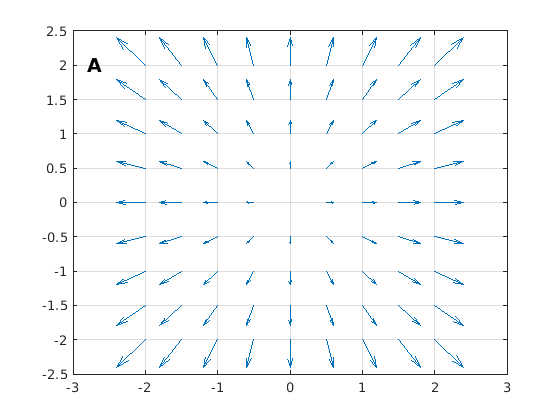
\includegraphics[width=8cm]{17_vector_calculus/vect_field1}
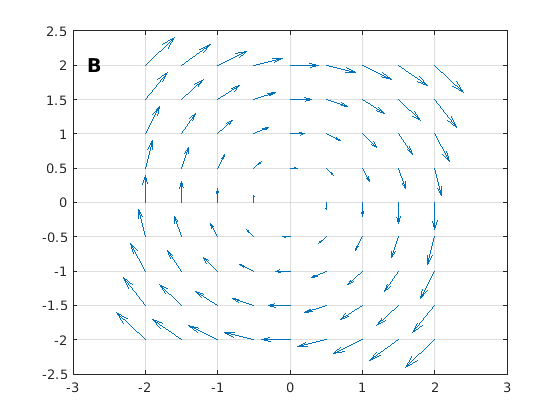
\includegraphics[width=8cm]{17_vector_calculus/vect_field2}

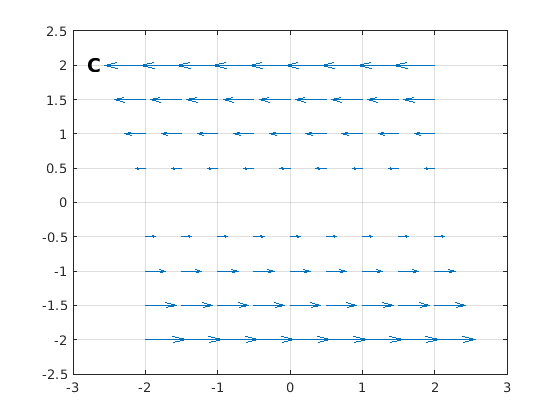
\includegraphics[width=8cm]{17_vector_calculus/vect_field3}
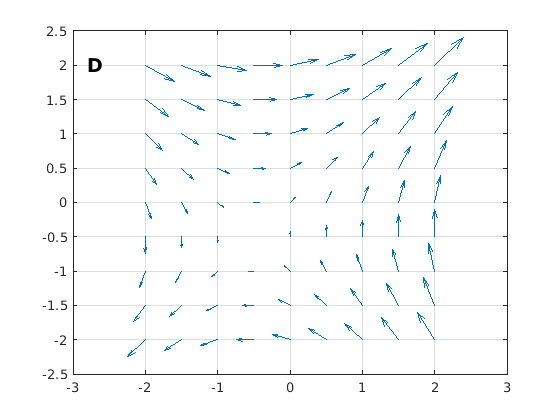
\includegraphics[width=8cm]{17_vector_calculus/vect_field4}
\label{17Q8}
\end{question}

\subsection{Intégrale sur une surface}

\begin{question}
Évaluez l'intégrale $\displaystyle \iint_S xy \dx{S}$ où $S$
est la surface du cylindre $y^2 + z^2 = 4$ entre les surface $y=0$ et
$y = 3 - x$.
\label{17Q9}
\end{question}

\begin{question}
Évaluez l'intégrale $\displaystyle \iint_S (x^2+y^2)z \dx{S}$ où $S$
est la surface de la partie supérieure de la sphère de rayon $2$
centrée à l'origine qui est à l'intérieur du cylindre de rayon
$\sqrt{2}$ dont l'axe principal est l'axe des $z$.
\label{17Q10}
\end{question}

\begin{question}
Quelle est la masse de l'entonnoir donnée par l'équation
$z = 2 \sqrt{x^2+y^2}$ dont le rayon de la base de l'entonnoir est $1$
et le rayon du dessus de l'entonnoir est $3$.  La densité est donnée
par $\rho(x,y,z) = 8 - z$.
\label{17Q11}
\end{question}

\begin{question}
Quelle est l'aire de la partie de la paraboloïde $y = x^2 + z^2$ qui
est à l'intérieur du cylindre $x^2 + z^2 = 9$.
\label{17Q12}
\end{question}

\begin{question}
Quelle est l'aire de la partie de la paraboloïde $z = x^2 + y^2 - 4$ qui
est à l'intérieur du cylindre $x^2 + y^2 = 1$.
\label{17Q13}
\end{question}

\begin{question}
Calculez l'aire de la surface $S$ du solide obtenu par l'intersection de
la balle $x^2 + y^2 + z^2 \leq 8$ et de la région $z \geq (x^2 + y^2)/2$.
\label{17Q14}
\end{question}

\begin{question}
Calculez l'aire de la partie $S$ du cylindre $x^2 + z^2 = a^2$ qui se
trouve à l'intérieur du cylindre $x^2 + y^2 = a^2$.  Dessinez cette
surface.
\label{17Q15}
\end{question}

\begin{question}
Calculez l'aire de la partie $S$ de la surface de la sphère d'équation
$x^2 + y^2 + z^2 = a^2$ qui se trouve à l'intérieur du cylindre
$x^2 + y^2 = ax$.  Dessinez cette surface.
\label{17Q16}
\end{question}

\begin{question}
Calculez l'intégrale $\displaystyle \iint_S F \cdot \dx{\VEC{S}}$
où $F(x,y,z) = (x,y,z)$ et $S$ est la partie du paraboloïde
$z = x^2+y^2$ pour $z\leq 4$.  L'orientation sur la surface $S$ est
donnée par un vecteur normal unitaire qui point dans la direction
de $z$ positif.
\label{17Q17}
\end{question}

\begin{question}
Calculez le flux du champ de vecteur $F(x,y,z) = (xy,y^2,yz)$
qui passe au travers de la partie de la sphère de rayon $2$ centrée à
l'origine qui se trouve dans la région $y\geq 0$.  L'orientation sur
la sphère est donnée par un vecteur normal unitaire dans la direction
de $y$ positif.
\label{17Q18}
\end{question}

\begin{question}
Calculer le flux du champ de vecteurs
$F(x,y,z) = -x\ii - y\jj + z^2\kk$  au travers de la partie du
cône $z=\sqrt{x^2+y^2}$ qui se trouve entre les plans $z=2$ et $z=3$.
L'orientation de la surface est donnée par la normale qui pointe
dans la direction de $z$ négatif.
\label{17Q19}
\end{question}

\begin{question}
Calculez le flux du champ de vecteur $F(x,y,z) = (y,x,z)$
qui passe au travers de l'hélicoïde $S$ décrit par la représentation
paramétrique
\[
  \rho(u,v) = (u \cos(v) , u \sin(v), v)
\]
pour $(u,v) \in D = \{(u,v) : 0\leq u \leq 1,\ 0\leq v \leq 2\pi \}$.
L'orientation de la surface est donnée par le vecteur normal unitaire
$\VEC{n}$ qui pointe dans la direction de $z$ positif.
\label{17Q20}
\end{question}

\begin{question}
Soit $F(x,y,z) = (x, \cos(xy) , z)$ et $S$ la surface du
cylindre $x^2+z^2 = a^2$ qui se trouve à l'intérieur du cylindre
$y^2+z^2=a^2$.  L'orientation sur $S$ est donnée par un vecteur
unitaire normal qui pointe vers l'extérieur du cylindre
$x^2 + z^2 = a^2$.  Calculez
$\displaystyle \iint_S F \cdot \dx{\VEC{S}}$.
\label{17Q21}
\end{question}

\subsection{Théorèmes de Stokes et de Green}

\begin{question}
Utilisez le Théorème de Green pour évaluez l'intégrale
$\displaystyle \int_C(2xy -x^2)\dx{x} + (x + y^2)\dx{y}$
où $C$ est la frontière de la région $D$ du premier quadrant
(c'est-à-dire, $x,y \geq 0$) définie par $x^2 + y^2 \leq 1$.
L'orientation de $C$ est dans le sens contraire aux aiguilles d'une
montre.
\label{17Q22}
\end{question}

\begin{question}
Évaluez l'intégrale
$\displaystyle \int_C(y+e^{x^2})\dx{x} + (2x + \cos(y^2))\dx{y}$
où $C$ est la frontière de la région $D$ bornée par les courbes
$y=x^2$ et $x = y^2$.  L'orientation de $C$ est dans le sens contraire
aux aiguilles d'une montre.
\label{17Q23}
\end{question}

\begin{question}
Nous voulons déplacer une particule le long de la courbe $C$ qui part de
l'origine pour se rendre au point $(2,0)$ en longeant l'axe des $x$,
puis se rendre au point $(-2,0)$ en longeant la partie supérieure du
cercle $x^2 + y^2 = 4$, et finalement revenir à l'origine encore en
longeant l'axe des $x$.  Calculez le travail nécessaire pour déplacer
un particule le long de ce trajet si le champ de vecteurs est
$F = (x, x^3 + 3 xy^2)$.
\label{17Q24}
\end{question}

\begin{question}
Soit $F(x,y,z) = (yz, xy, xz)$ et $C$ le rectangle de sommets
aux points $(0,0,2)$, $(1,0,2)$, $(1,1,2)$ et $(0,1,2)$.   Supposons
que $C$ soit parcourue dans le sens contraire aux aiguilles d'une
montre lorsque nous l'observons d'un point $(0,0,z)$ avec $z>2$.
Utilisez le Théorème de Stokes pour calculer l'intégrale
$\displaystyle \int_C F \cdot \dx{\VEC{s}}$.
\label{17Q25}
\end{question}

\begin{question}
Soit $F(x,y,z) = (y^2, x, z)$.  Utilisez le Théorème de Stokes
pour calculer l'intégrale
$\displaystyle \int_C F \cdot \dx{\VEC{s}}$
où $C$ est la courbe donnée par l'intersection du cylindre d'équation
$x^2 + y^2 =4$ et du plan contenant les points $(0,2,0)$, $(1,1,1)$ et
$(-1,1,2)$.  L'orientation sur $C$ est dans le sens des aiguilles
d'une montre lorsque vue du dessus (i.e.\ d'un point $(0,0,z)$ pour
$z>0$ très grand).
\label{17Q26}
\end{question}

\begin{question}
Soit $S$ la surface de la paraboloïde $z = 4 - x^2 - y^2$ qui se
trouve dans la région $x,y,z \geq 0$.  Calculez
$\displaystyle \int_C F \cdot \dx{\VEC{s}}$ où le champ de
vecteur $F$ est défini par
$F(x,y,z) = -yz(1-z) \, \ii + xz \, \jj + xyz \, \kk$
et la direction sur la courbe $C = \partial S$ est dans le sens
contraire aux aiguilles d'une montre lorsque que vu d'un point sur
l'axe des $z$ avec $z > 4$.
\label{17Q27}
\end{question}

\begin{question}
Soit $F(x,y,z) = x\; \ii + y\;\kk$ et $S$ la partie du
paraboloïde d'équation $z = x^2+y^2$ pour $z \leq 4$.  L'orientation
sur $S$ est donnée par un vecteur unitaire qui pointe dans la
direction de $z$ positif.  Calculez
$\displaystyle \iint_S \curl F \cdot \dx{\VEC{S}}$.
\label{17Q28}
\end{question}

\begin{question}
Soit $F(x,y,z) = z^3 e^{xz^2}\, \ii + z^4 e^{yz^2}\, \jj + xy\,\kk$ et
$S$ la surface du cylindre $x^2+y^2 = 4$ pour $2 \leq z \leq 4$.
L'orientation sur $S$ est donnée par un vecteur unitaire normal qui
pointe vers l'extérieur du cylindre.  Calculez
$\displaystyle \iint_S \curl  F \cdot \dx{\VEC{S}}$.
\label{17Q29}
\end{question}

\subsection{Théorème de la divergence}

\begin{question}
Soit $F(x,y,z) = (x+y)\ii + (y+z) \jj + (x + z) \kk$ et
$S$ la surface du tétraède bornée par les plans $x=0$, $y=0$, $z=0$ et
$x+y+z=1$.  L'orientation de $S$ est donnée par une normale unitaire à
$S$ qui pointe vers l'extérieure.  Calculez
$\displaystyle \iint_S F \cdot \dx{\VEC{S}}$ à l'aide du
Théorème de la divergence.
\label{17Q30}
\end{question}

\begin{question}
Soit $F(x,y,z) = x^3\ii + y^3 \jj + (z^3 + \cos(y^2)) \kk$ et
$E$ le solide délimité par le cylindre $x^2+y^2 =1$ et les plans $z=0$
et $z=2$.  L'orientation sur la surface $S$ de $E$ est donnée par une
normale unitaire qui pointe vers l'extérieure.  Calculez le flux de
$F$ qui s'échappe de ce solide; c'est-à-dire, calculez
$\displaystyle \iint_S F \cdot \dx{\VEC{S}}$.
\label{17Q31}
\end{question}

\begin{question}
Soit $F(x,y,z) = xy^2\,\ii + 2xz^2\, \jj + x^2 z\, \kk$ et
$E$ le solide délimité par le paraboloïde $z = 4 - x^2 - y^2$ et le
plan $z=0$.  L'orientation sur la surface $S$ de $E$ est donnée par la
normale unitaire qui pointe vers l'extérieure.  Calculez le flux de
$F$ qui s'échappe de ce solide; c'est-à-dire, calculez
$\displaystyle \iint_S F \cdot \dx{\VEC{S}}$.
\label{17Q32}
\end{question}


%%% Local Variables: 
%%% mode: latex
%%% TeX-master: "notes"
%%% End: 
